\documentclass[letterpaper, 12pt]{article}
% \usepackage[showframe, margin=1in, top=0.25in, bottom=0.25in, includeheadfoot, headheight=0.5in]{geometry}
\usepackage[margin=1in, top=0.25in, bottom=0.25in, includeheadfoot, headheight=0.5in]{geometry}

\AddToHook{cmd/section/before}{\clearpage}

\usepackage[table]{xcolor}
\colorlet{listingback}{gray!20}
\definecolor{headingcolor}{RGB}{110,34,54}

\usepackage{fancyhdr}
\renewcommand{\sectionmark}[1]{\markboth{#1}{#1}}

% Used to detect whether a section is an appendix to print the right thing in the footer
\usepackage{etoolbox}
\newtoggle{inappendix}
\pretocmd{\appendix}{\clearpage\toggletrue{inappendix}}{}{}

% Save standard definitions for head and foot rules (lines separating header and footer from text)
\let\HeadRule\headrule
\let\FootRule\footrule
% Add color to the standard definitions
\renewcommand{\headrule}{\color{headingcolor}\HeadRule}
\renewcommand{\footrule}{\textcolor{headingcolor}{\FootRule}}

% IMPORTANT: This command should not be called directly. Use \preamble.
% Macro to insert the title page for each lab.
% The argument is the title of the lab.
\newcommand{\inserttitlepage}[1]
{
    \begin{titlepage}
    \centering
    
\includegraphics[scale=0.5]{images/nexus_lab_logo.png}

    \vspace*{\baselineskip}

    \textbf{\Large OpenStack Labs}

    \vspace*{\baselineskip}

    \textbf{\Large #1}
    \vspace*{\fill}
\end{titlepage}
}

% IMPORTANT: This command should not be called directly. Use \preamble.
% Macro to define header and footer for each lab.
% The argument is the title of the lab.
\newcommand{\headfoot}[1]
{
    \fancypagestyle{fancy}
    {
        \fancyhf{}
        \fancyhead[L]{\footnotesize #1}
        \fancyhead[R]{
\includegraphics[height=0.85\headheight]{images/nexus_lab_logo.png}}
        \fancyfoot[L]{%
            \footnotesize%
            \ifnum\value{section}>0%
            \iftoggle{inappendix}{Appendix \thesection: \rightmark}{Section \thesection: \rightmark}%
            \fi}
        \fancyfoot[R]{\footnotesize\thepage}
        \renewcommand{\headrulewidth}{1.5pt}
        \renewcommand{\footrulewidth}{1.5pt}
    }
}

% Macro to insert title page, define header and footer, and insert table of contents and about section for each lab.
% The argument is the title of the lab.
\newcommand{\preamble}[1]
{
    \pagenumbering{roman}
    \inserttitlepage{#1}
    \headfoot{#1}

    % Insert table of contents
    \pagestyle{fancy}
    \tableofcontents
    \clearpage

    \section*{About This Document}
    \label{sec:about_this_document}
    \begin{itemize}
        \item This document was developed by a team at the University of Tennessee at Chattanooga led by Dr. Mengjun Xie
        (\href{mailto:mengjun-xie@utc.edu}{\textbf{mengjun-xie@utc.edu}}).
        \item The development of this document was supported by a National Centers of Academic Excellence in Cybersecurity Grant (\#H98230-20-1-0351), housed at the National Security Agency.
        \item This document is licensed with a Creative Commons Attribution 4.0 International License.
    \end{itemize}
    \clearpage
}

% Macro to insert the Lab Settings page for each lab. Call after the Introduction and Objectives sections.
\newcommand{\labsettings}
{
    \section*{Lab Settings}
    \label{sec:lab_settings}
    \addcontentsline{toc}{section}{\nameref{sec:lab_settings}}
    The information in the table below will be needed in order to complete the lab.
    The task sections below provide details on the use of this information.
    \begin{table*}[htbp]
        \centering
        \begin{tabular}{|c|c|c|c|}
            \hline
            \rowcolor{gray!20} \textbf{Virtual Machine} & \textbf{IP Address} & \textbf{Account} & \textbf{Password} \\
            \hline
            \multirow{2}{*}{\texttt{workstation}} & \multirow[t]{2}{*}{\texttt{ens3: 192.168.1.21}}  & \multirow{2}{*}{\texttt{ubuntu}} & \multirow{2}{*}{\texttt{ubuntu}} \\
                                                  & \multirow[t]{2}{*}{\texttt{ens4: 172.25.250.21}} &                                  &                                  \\
            \hline
            \multirow{2}{*}{\texttt{devstack}}    & \multirow[t]{2}{*}{\texttt{ens3: 192.168.20}}    & \multirow{2}{*}{\texttt{ubuntu}} & \multirow{2}{*}{\texttt{ubuntu}} \\
                                                  & \multirow[t]{2}{*}{\texttt{ens4: 172.25.250.20}} &                                  &                                  \\
            \hline
        \end{tabular}
    \end{table*}
    \clearpage

    % IMPORTANT(lucas): If another frontmatter section ever gets placed after this, this command needs to be moved
    % to the end of that section.
    % I have placed this here and not in each lab purely for convenience and to ensure I don't forget any.
    \pagenumbering{arabic}
}

% Sans-serif font
\renewcommand{\familydefault}{\sfdefault}
\newcommand{\texttildemid}{{\raisebox{0.5ex}{\texttildelow}}}

\usepackage{enumitem}
\renewcommand{\labelenumi}{\textbf{\thesection.\arabic{enumi}.}}

% Try to forbid widows and orphans
\widowpenalty10000
\clubpenalty10000

\usepackage{graphicx}
\usepackage{hyperref}
\hypersetup{colorlinks=true,linkcolor=black,urlcolor={[named] headingcolor}}

\usepackage{sectsty}
\sectionfont{\color{headingcolor}}

% Table of Contents
\usepackage{bookmark}
\usepackage[titles]{tocloft}
\usepackage[title]{appendix}
\renewcommand{\cfttoctitlefont}{\Large\bfseries\color{headingcolor}}
\renewcommand{\cftsecfont}{\normalfont\normalsize}
\renewcommand{\cftsecpagefont}{\normalfont\normalsize}
\renewcommand{\cftdotsep}{0} % Make dots small and close together
\renewcommand{\cftsecleader}{\cftdotfill{\cftdotsep}} % Add dots after section titles
% Make dots go all the way to the page number
\renewcommand{\cftsecfillnum}[1]{{\cftsecleader}\nobreak{\cftsecpagefont #1}\cftsecafterpnum\par}

\usepackage{multirow}
\setlength{\tabcolsep}{16pt}
\renewcommand{\arraystretch}{1.1}

% For nice-looking boxes
\usepackage[most]{tcolorbox}
\usepackage{listings}
\usepackage{lstautogobble}
\lstset{
  frame=none,
  language=Bash,
  showstringspaces=false,
  basicstyle={\linespread{1.1}\footnotesize\ttfamily\selectfont},
  numbers=none,
  breaklines=true,
  breakatwhitespace=true,
  tabsize=3,
  columns=fullflexible,
  keepspaces=true,
  escapeinside={(*@}{@*)},
  literate={~}{{\texttildemid}}{1}
           {\#}{\#}{1},
  autogobble=true
}

\tcolorboxenvironment{lstlisting}
{
    spartan,
    colframe=gray!50,
    boxsep=0mm,
    left=1mm,
    right=1mm,
    top=-1mm,
    bottom=-1mm,
    colback=gray!20
}

% Hacky solution for now, would like to have just one environment and make several tcolorboxes by passing different
% colors as parameters, but that is giving errors
\makeatletter
\tcbset{
  note/.style={%
        enhanced,
        breakable,
        colback=blue!10!white,
        colframe=blue!80!white,
        attach boxed title to top left={yshift*=-\tcboxedtitleheight},
        title={#1},
        boxed title size=title,
        boxed title style={%
            sharp corners,
            rounded corners=northwest,
            colback=tcbcolframe,
            boxrule=0pt,
        },
        underlay boxed title={%
            \path[fill=tcbcolframe] (title.south west)--(title.south east)
                to[out=0, in=180] ([xshift=5mm]title.east)--
                (title.center-|frame.east)
                [rounded corners=\kvtcb@arc] |-
                (frame.north) -| cycle;
        },
    }
}
\makeatother

\makeatletter
\tcbset{
    stop/.style={%
        enhanced,
        breakable,
        colback=white,
        colback=red!10!white,
        colframe=red!80!white,
        attach boxed title to top left={yshift*=-\tcboxedtitleheight},
        title={#1},
        boxed title size=title,
        boxed title style={%
            sharp corners,
            rounded corners=northwest,
            colback=tcbcolframe,
            boxrule=0pt,
        },
        underlay boxed title={%
            \path[fill=tcbcolframe] (title.south west)--(title.south east)
                to[out=0, in=180] ([xshift=5mm]title.east)--
                (title.center-|frame.east)
                [rounded corners=\kvtcb@arc] |-
                (frame.north) -| cycle;
        },
    }
}
\makeatother

\makeatletter
\tcbset{
    tip/.style={%
        enhanced,
        breakable,
        colback=white,
        colback=green!10,
        colframe=green!70!black,
        attach boxed title to top left={yshift*=-\tcboxedtitleheight},
        fonttitle=\bfseries,
        title={#1},
        boxed title size=title,
        boxed title style={%
            sharp corners,
            rounded corners=northwest,
            colback=tcbcolframe,
            boxrule=0pt,
        },
        underlay boxed title={%
            \path[fill=tcbcolframe] (title.south west)--(title.south east)
                to[out=0, in=180] ([xshift=5mm]title.east)--
                (title.center-|frame.east)
                [rounded corners=\kvtcb@arc] |-
                (frame.north) -| cycle;
        },
    }
}
\makeatother

% The commands below define environments for colored boxes. They are used like
% \begin{notebox}
% ...
% \end{notebox}
\newtcolorbox{notebox}{note={Note}}
\newtcolorbox{stopbox}{stop={Stop}}
\newtcolorbox{tipbox}{tip={Tip}}

\begin{document}
\preamble{Lab 07: Managing an OpenStack Instance}

\section*{Introduction}\label{sec:introduction}
\addcontentsline{toc}{section}{\nameref{sec:introduction}}
Up to this point, whenever you have launched an instance, its resources and running state have remained mostly constant.
However, OpenStack instances are quite flexible, even after being launched.
In this lab, you will launch an instance and perform several management operations while it is running.

\section*{Objectives}\label{sec:objectives}
\addcontentsline{toc}{section}{\nameref{sec:objectives}}
\begin{itemize}[itemsep=0pt]
    \item Create a snapshot of an instance.
    \item Manage the running and power state of an instance.
    \item Shelving and Rescuing an instance.
\end{itemize}
\clearpage

\labsettings

%%%%%%%%%%%
% Section 1
%%%%%%%%%%%
\section{Creating a Snapshot with the Horizon Dashboard}\label{sec:creating-a-snapshot-web}
In this task, you will launch an instance, modify its configuration, and make a snapshot of it for later use.
Taking a snapshot of an image captures its state and data on disk.
An OpenStack snapshot can be used as an image to launch other instances.
Snapshots are useful tools in many situations.
One is to aid in the backup of instance or as a precaution before a major change so that the image is easily recoverable.
Another use of snapshots is to build off an existing image to create a better template for new instances.
For instance, consider the case where you want to launch multiple customized FTP servers.
Instead of launching each one from a basic Ubuntu image and modifying their configurations individually, you might set up one instance completely and take a snapshot.
That snapshot could then be used as a template for the other instances to save time and prevent mistakes.

\begin{enumerate}
    \begin{labstep}
        Log in to the \textbf{workstation} machine as the \textbf{ubuntu} user with password \textbf{ubuntu}.

        \begin{center}
            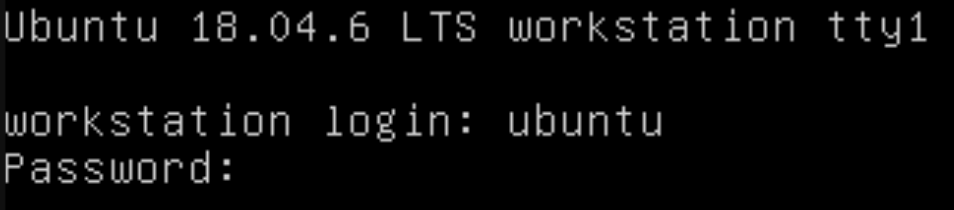
\includegraphics[width=\linewidth]{images/part1/step1.png}
        \end{center}
    \end{labstep}

    \begin{labstep}
        Launch the graphical user interface.
        \begin{lstlisting}
            ubuntu@workstation:~$ startx
        \end{lstlisting}

        \begin{center}
            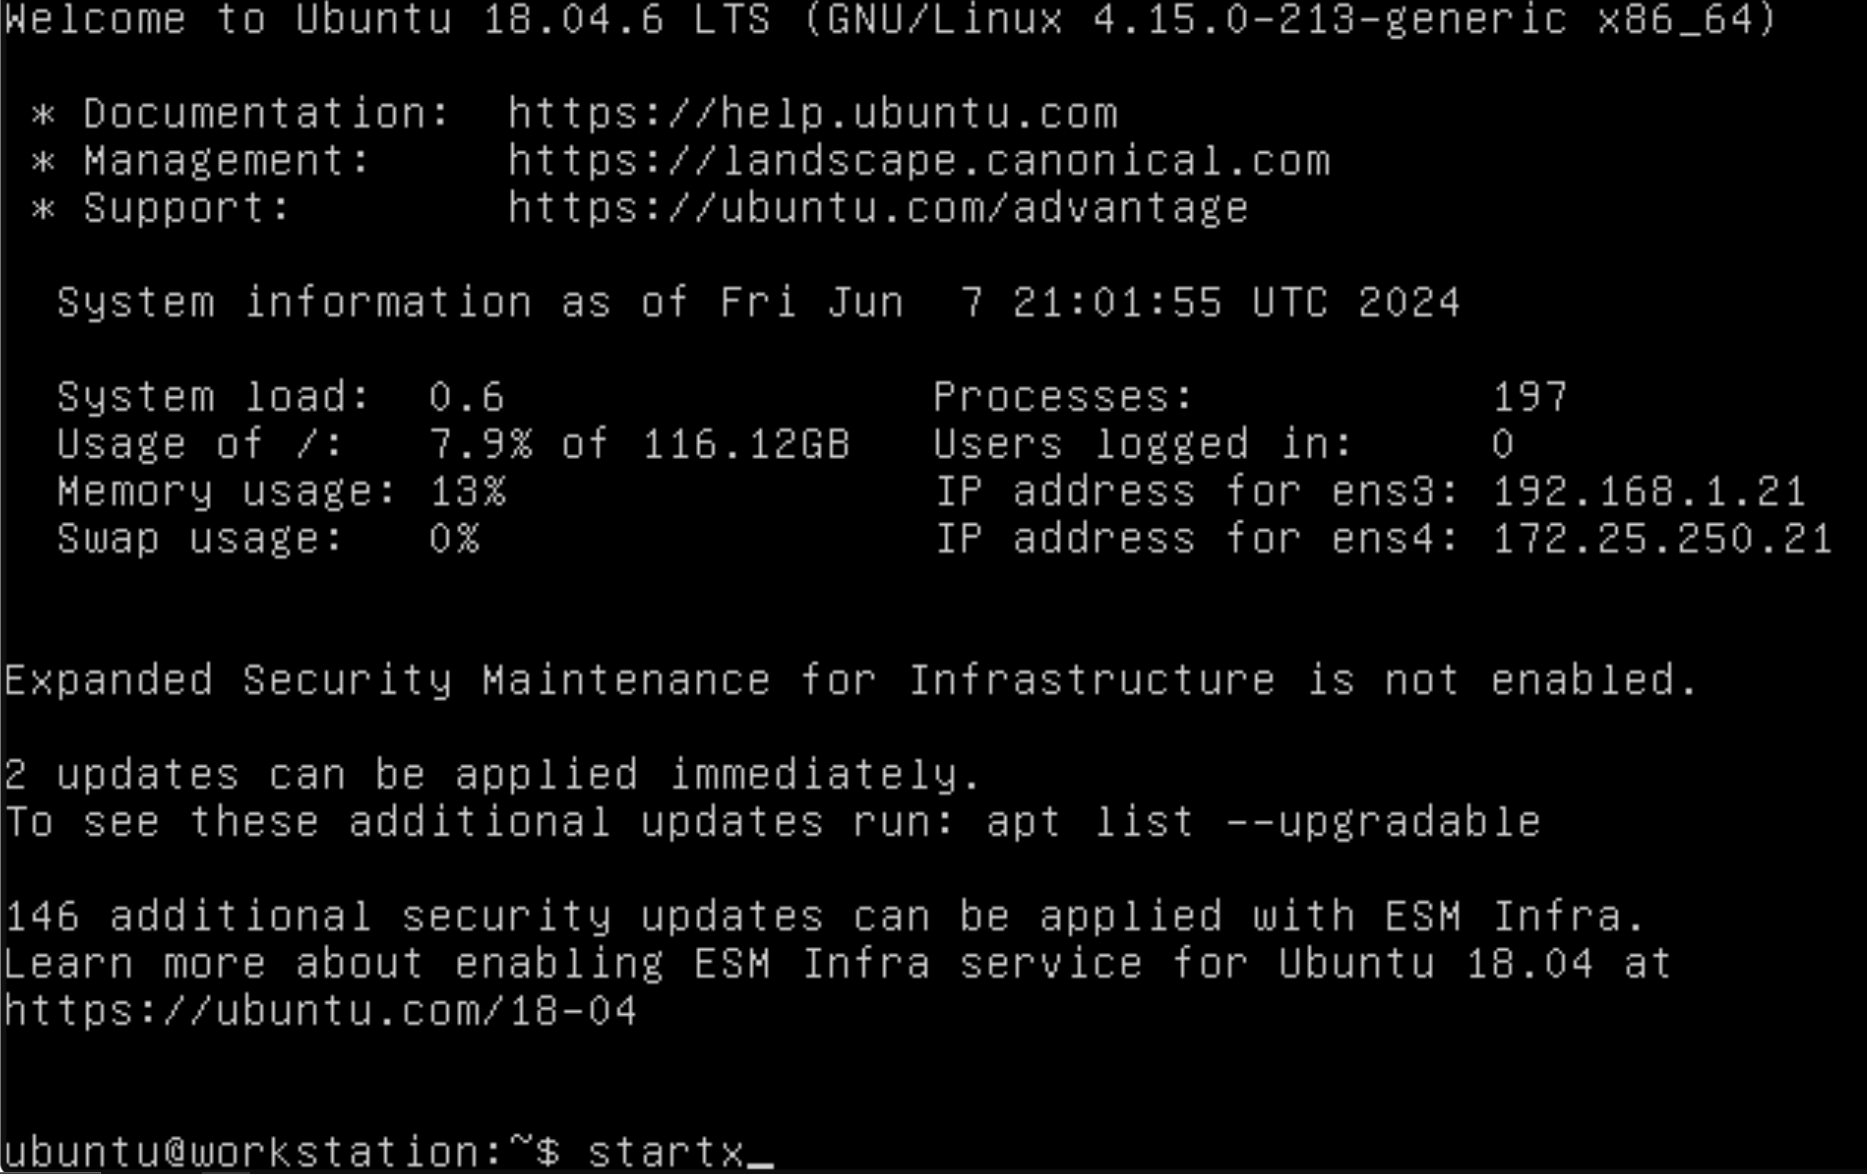
\includegraphics[width=\linewidth]{images/part1/step2.png}
        \end{center}
    \end{labstep}

    \begin{labstep}
        Open the web browser, and navigate to \textbf{192.168.1.20}.
        Log in to the dashboard as \textbf{admin} with the password \textbf{secret}.

        \begin{center}
            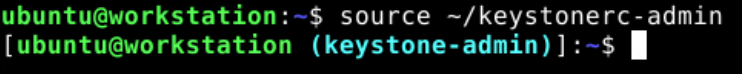
\includegraphics[scale=0.5]{images/part1/step3.png}
        \end{center}
    \end{labstep}

    \begin{labstep}
        Ensure the \textbf{demo} project is selected.
        Navigate to \textbf{Project $>$ Compute $>$ Instances}, and click \textbf{Launch Instance}.

        \begin{center}
            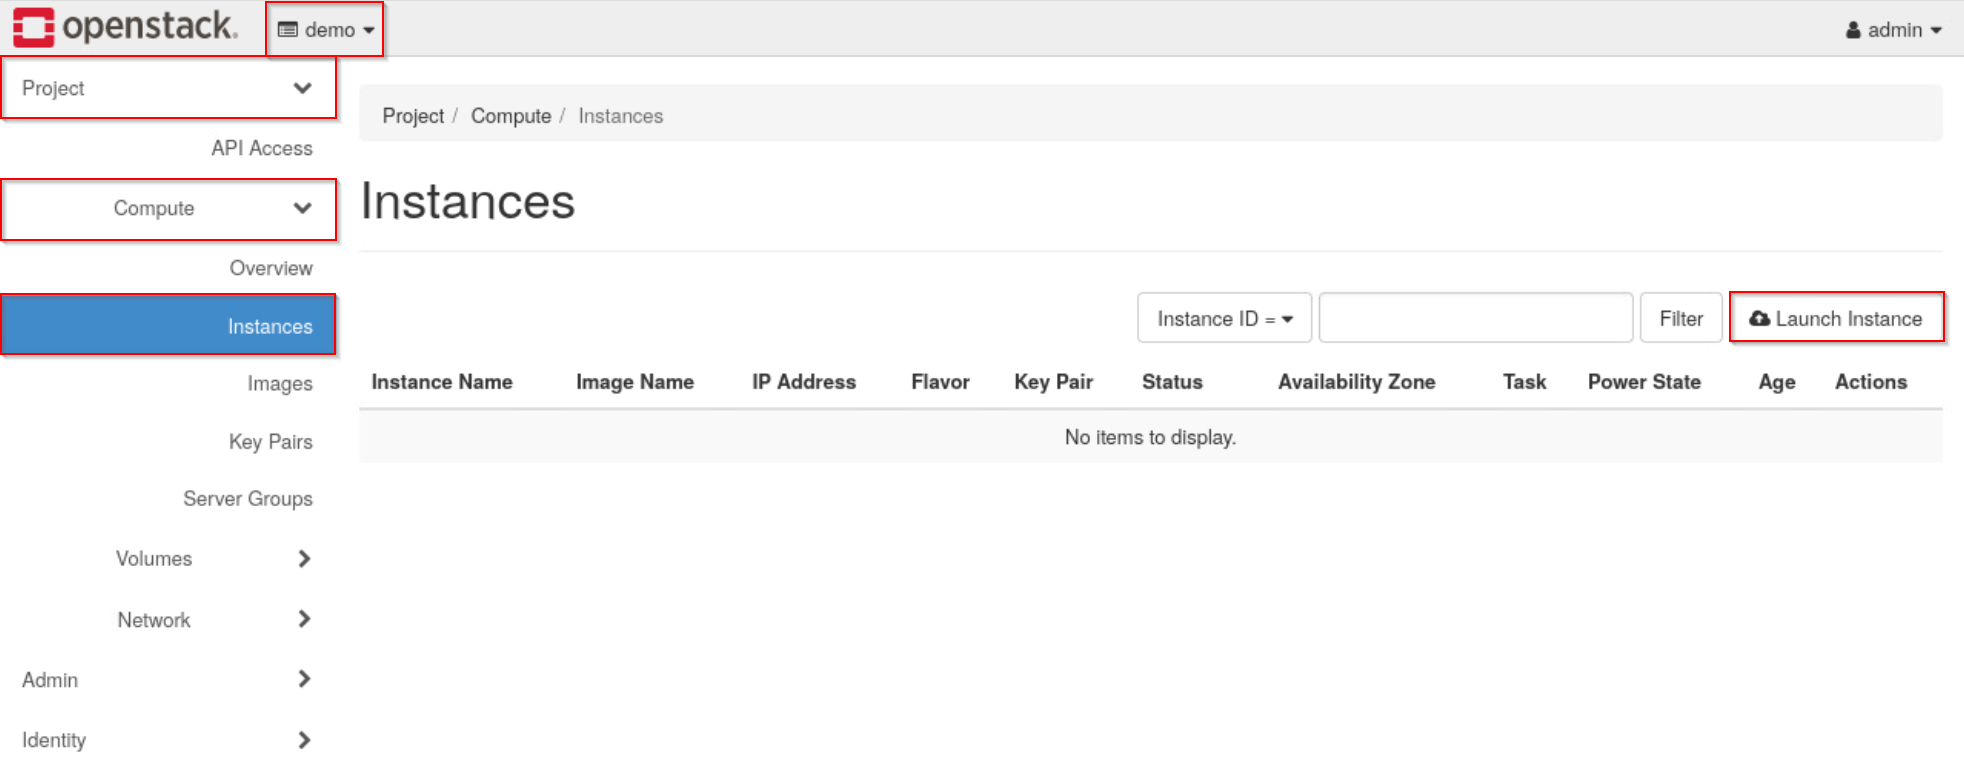
\includegraphics[width=\linewidth]{images/part1/step4.png}
        \end{center}
    \end{labstep}

    \begin{labstep}
        In the \textit{Details} tab, enter \textbf{instance1} in the \textit{Instance Name} field and click \textbf{Next}.

        \begin{center}
            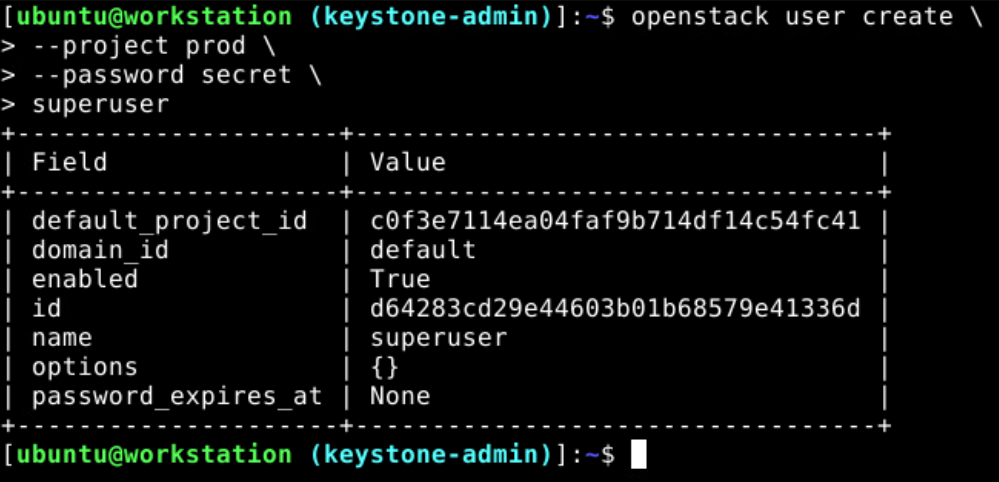
\includegraphics[width=\linewidth]{images/part1/step5.png}
        \end{center}
    \end{labstep}

    \begin{labstep}
        In the \textit{Source} tab, make sure \textbf{Image} is selected in the \textit{Select Boot Source} dropdown and select \textbf{No} under \textit{Create New Volume}.
        Select the \textbf{ubuntu} image by clicking the $\uparrow$ symbol in the same row.
        Click \textbf{Next}.

        \begin{center}
            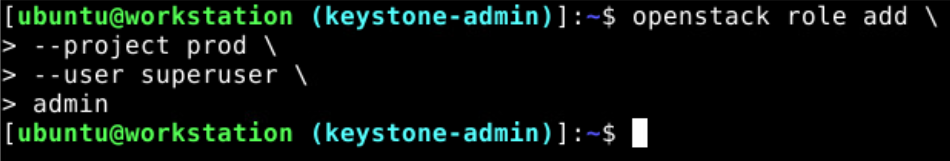
\includegraphics[width=\linewidth]{images/part1/step6.png}
        \end{center}
    \end{labstep}

    \begin{stopbox}
        Before proceeding to the next step, confirm that \textbf{ubuntu} appears underneath the \textit{Allocated} section.
    \end{stopbox}

    \begin{labstep}
        In the \textit{Flavor} tab, click the $\uparrow$ symbol in the same row as \textbf{m1.small}.
        Click \textbf{Next}.

        \begin{center}
            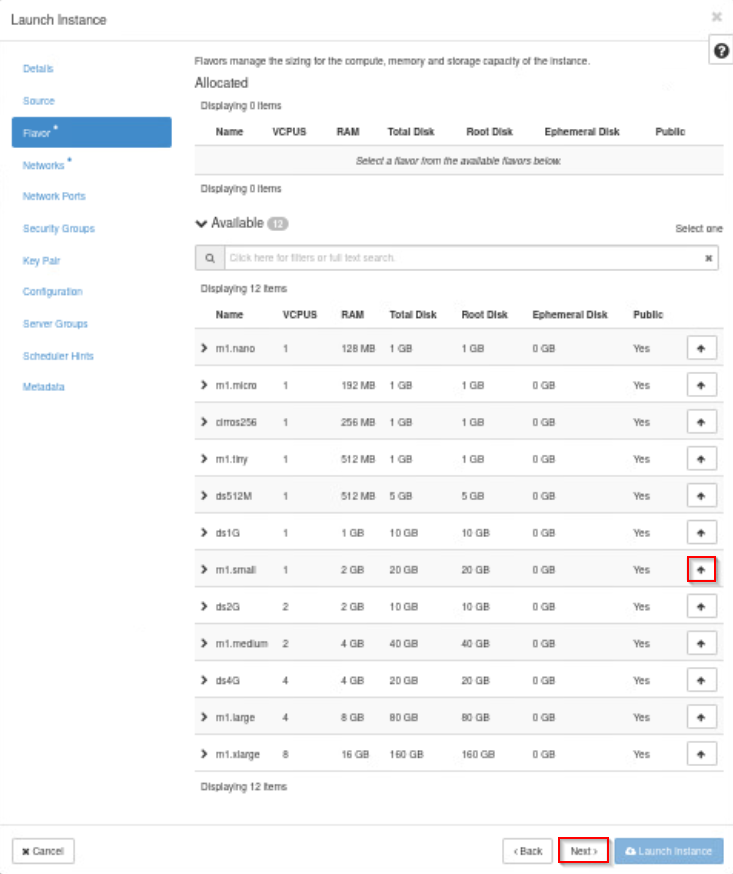
\includegraphics[width=\linewidth]{images/part1/step7.png}
        \end{center}
    \end{labstep}

    \begin{stopbox}
        Before proceeding to the next step, confirm that \textbf{m1.small} appears underneath the \textit{Allocated} section.
    \end{stopbox}

    \begin{labstep}
        In the \textit{Networks} tab, click the $\uparrow$ symbol in the same row as \textbf{shared}.
        Click \textbf{Launch Instance}.

        \begin{center}
            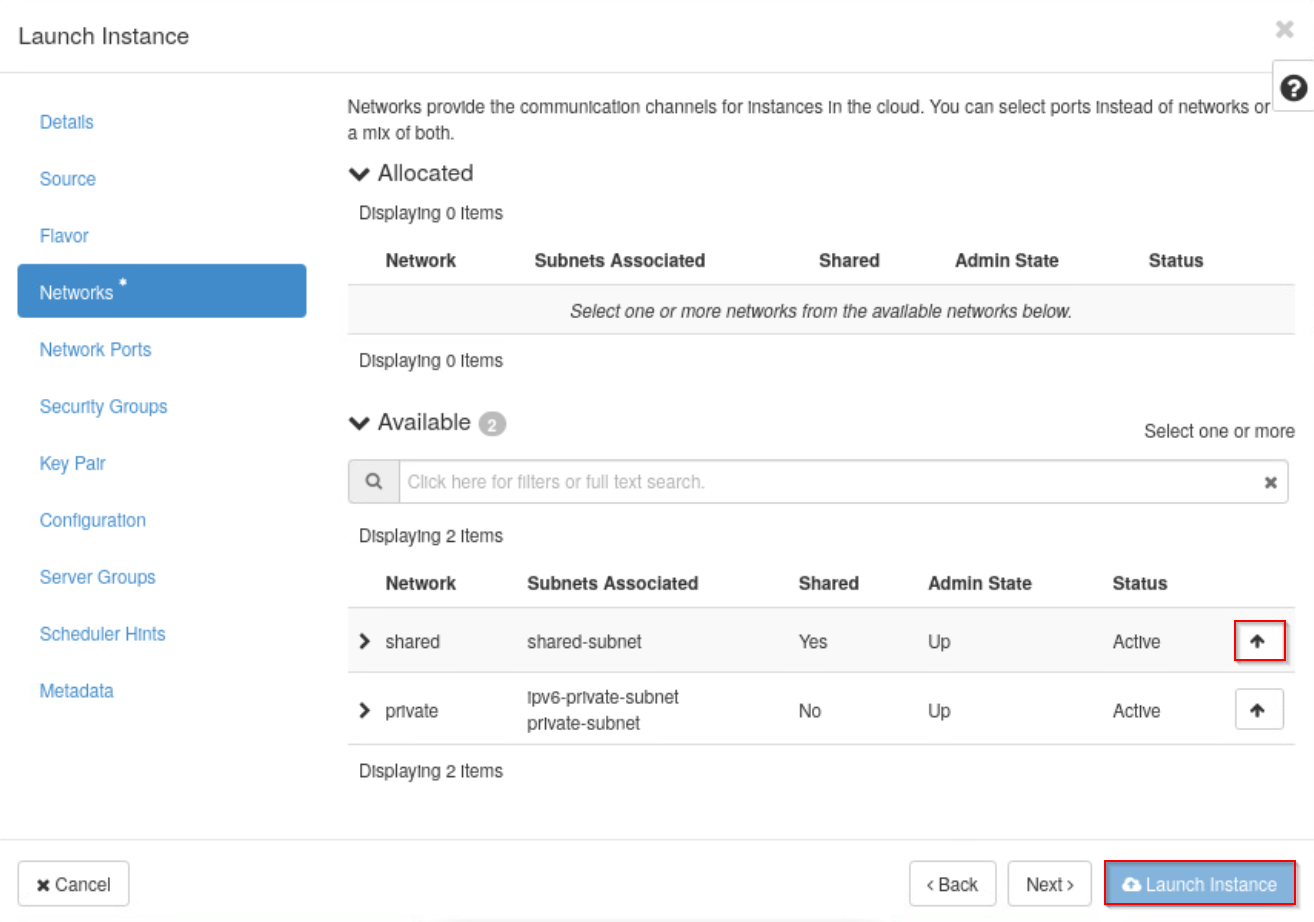
\includegraphics[width=\linewidth]{images/part1/step8.png}
        \end{center}
    \end{labstep}

    \begin{stopbox}
        Before proceeding to the next step, confirm that \textbf{shared} appears underneath the \textit{Allocated} section.
    \end{stopbox}

    \begin{labstep}
        Access the instance's console by clicking on \textbf{instance1} under the \textit{Instance Name} column.
        Then, navigate to the \textit{Console} tab if you are not directed there automatically.
        Click the \textbf{Click here to show only the console} link.

        \begin{center}
            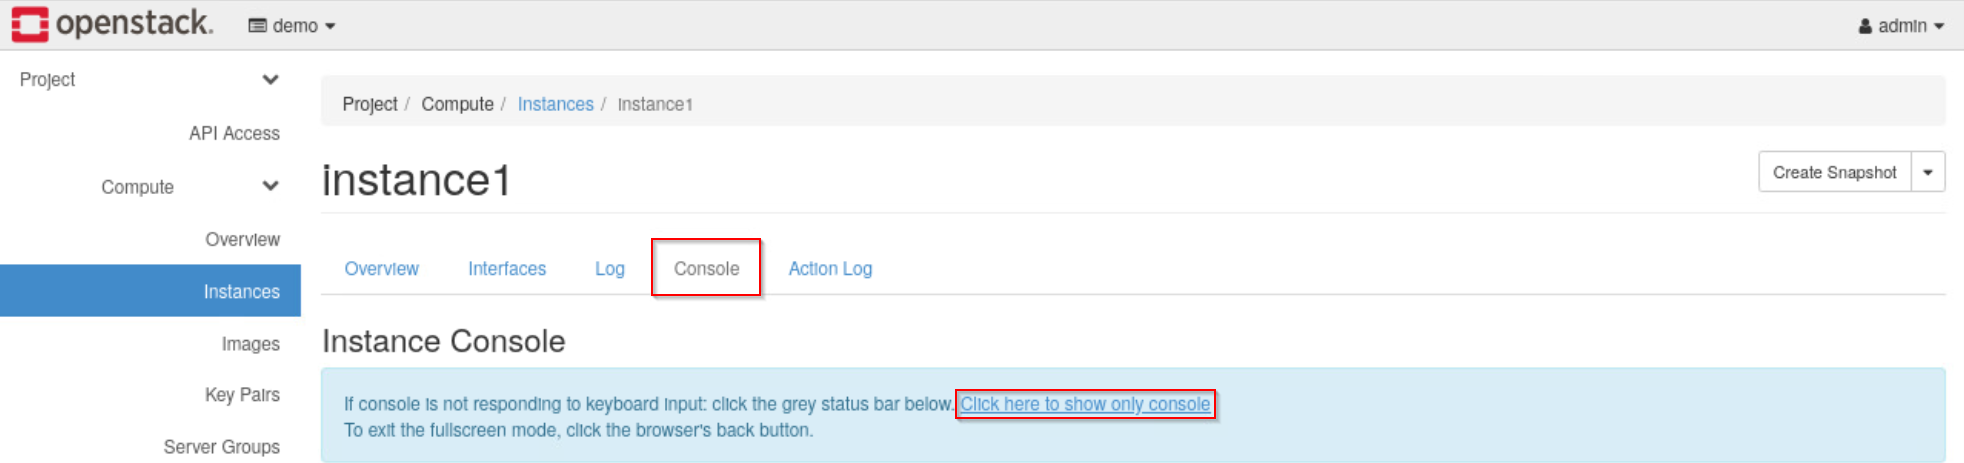
\includegraphics[width=\linewidth]{images/part1/step9.png}
        \end{center}
    \end{labstep}

    \begin{labstep}
        Log in to the instance as \textbf{root} with the password \textbf{secret}.

        \begin{center}
            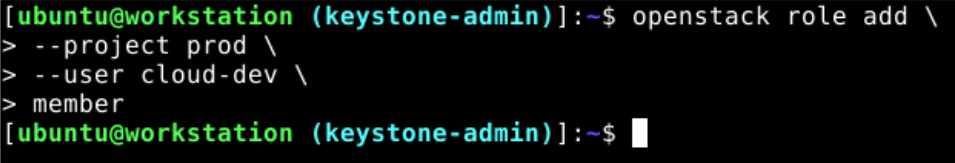
\includegraphics[width=\linewidth]{images/part1/step10.png}
        \end{center}
    \end{labstep}

    \begin{notebox}
        It may take several minutes for the instance to fully boot up and present a login prompt.
    \end{notebox}

    \begin{labstep}
        Now, we will make a change to the instance and create a snapshot.
        Create the \textbf{/root/hello.txt} file with the contents \textbf{Hello, world!}.
        \begin{lstlisting}
            root@instance1:~# echo 'Hello, world!' > /root/hello.txt
        \end{lstlisting}

        \begin{center}
            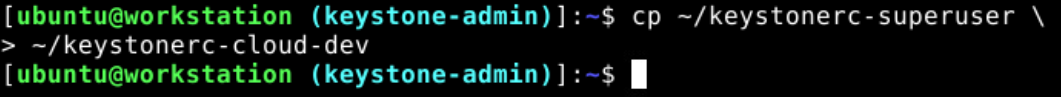
\includegraphics[width=\linewidth]{images/part1/step11.png}
        \end{center}
    \end{labstep}

    \begin{labstep}
        Now, navigate back to \textbf{Project $>$ Compute $>$ Instances}.
        Before creating a snapshot, click the dropdown next to \textbf{Create Snapshot} in the same row as \textbf{instance1}, then click \textbf{Shut Off Instance}.
        This will prevent any inconsistencies in the resulting snapshot.

        \begin{center}
            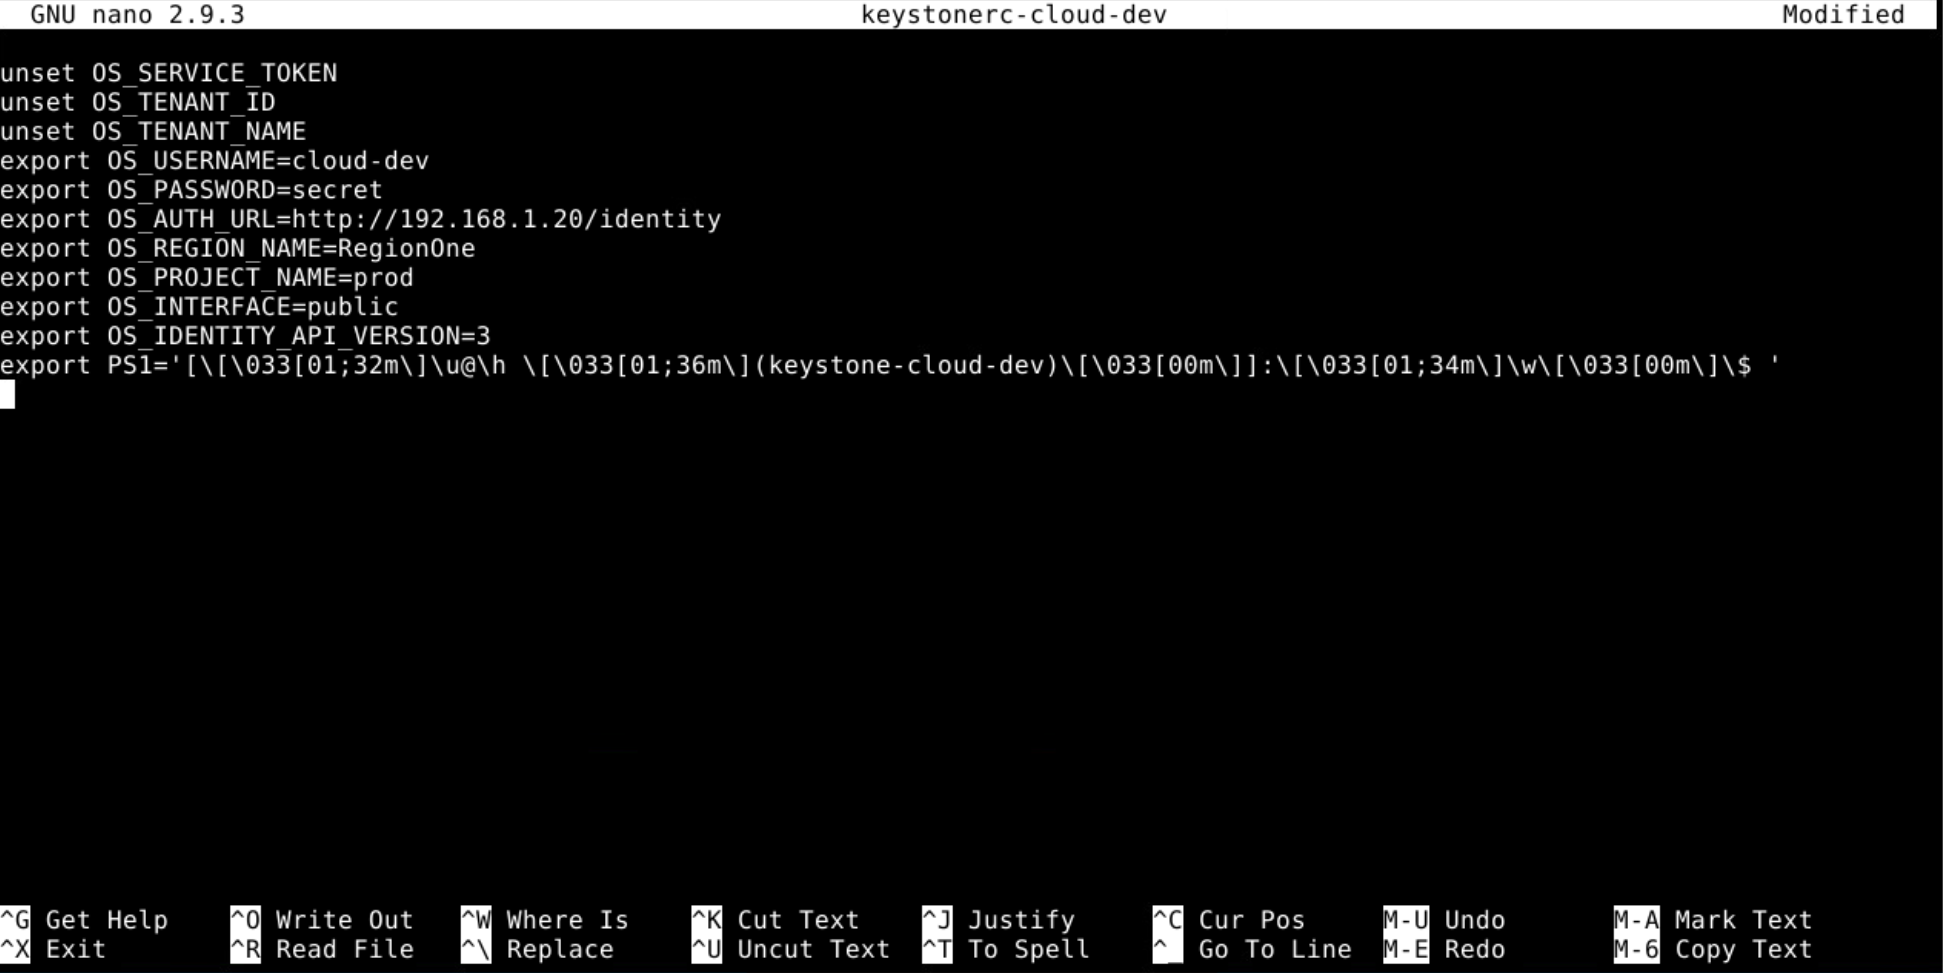
\includegraphics[width=\linewidth]{images/part1/step12.png}
        \end{center}
    \end{labstep}

    \begin{tipbox}
        A ``live snapshot'' is a snapshot of a running instance, which may only include a snapshot of the disk, while some OS state may be lost.
    \end{tipbox}
    \begin{notebox}
        Stopping instances and otherwise changing their running states will be explored further later in this lab.
    \end{notebox}

    \begin{labstep}
        When the \textit{Status} column shows that \textbf{instance1} is \textbf{Shutoff}, click \textbf{Create Snapshot}.

        \begin{center}
            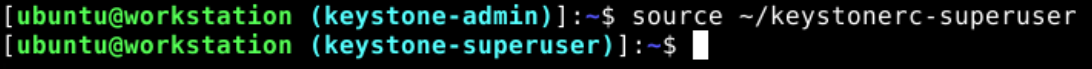
\includegraphics[width=\linewidth]{images/part1/step13.png}
        \end{center}
    \end{labstep}

    \begin{labstep}
        In the \textbf{Create Snapshot} dialog, enter \textbf{instance1-snapshot} in the \textit{Snapshot Name} field.
        Click \textbf{Create Snapshot}.

        \begin{center}
            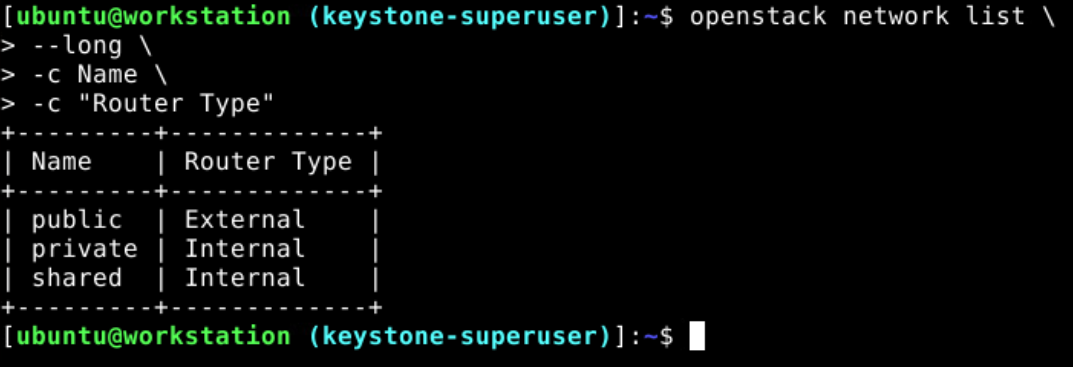
\includegraphics[width=\linewidth]{images/part1/step14.png}
        \end{center}
    \end{labstep}

    \begin{stopbox}
        When you create the snapshot, you will be redirected to \textbf{Projects $>$ Compute $>$ Images}.
        Wait until \textbf{instance1-snapshot} is \textbf{Active} before proceeding.
    \end{stopbox}

    \begin{labstep}
        Navigate back to the \textbf{Instances} page.
        The instance is no longer needed, so select the checkbox next to \textbf{instance1} and click \textbf{Delete Instances}.

        \begin{center}
            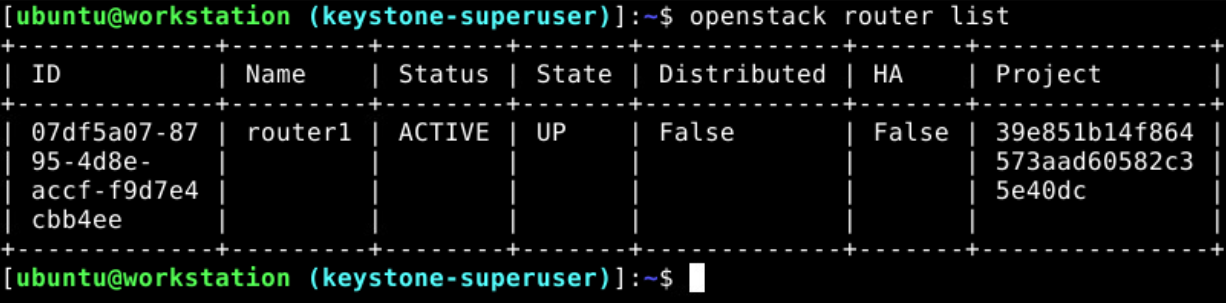
\includegraphics[width=\linewidth]{images/part1/step15.png}
        \end{center}
    \end{labstep}

    \begin{labstep}
        In the \textbf{Confirm Delete Instances} dialog, click \textbf{Delete Instances}.

        \begin{center}
            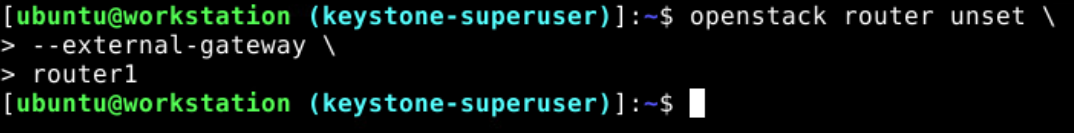
\includegraphics[width=\linewidth]{images/part1/step16.png}
        \end{center}
    \end{labstep}

    \begin{labstep}
        To verify that the snapshot works correctly, use the snapshot to launch another instance named \textbf{instance1}.
        Follow the same steps that were used to create \textbf{instance1}.
        However, in the \textit{Source} tab of the \textbf{Launch Instance} dialog, select \textbf{Image Snapshot} under \textit{Boot Source} click the $\uparrow$ symbol next to \textbf{instance1-snapshot}.

        \begin{center}
            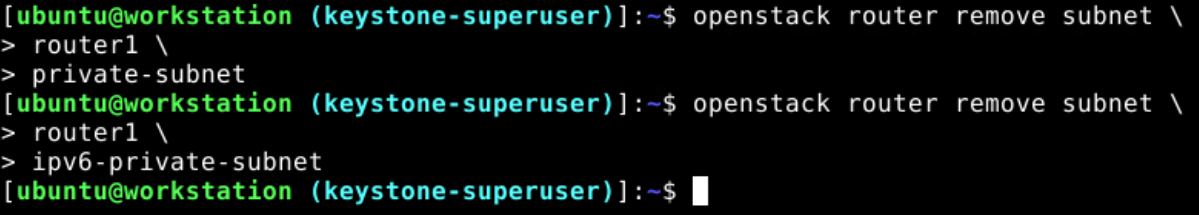
\includegraphics[width=\linewidth]{images/part1/step17.png}
        \end{center}
    \end{labstep}

    \begin{tipbox}
        The snapshot will also appear on the \textbf{Project $>$ Compute $>$ Images} page.
        It should say \textbf{Snapshot} in the \textit{Type} column.
        For an alternative method of launching an image with the snapshot, navigate to this page, click \textbf{Launch} in the same row as the snapshot, and enter the required information in the following dialog.
        The snapshot can also be deleted from here.
    \end{tipbox}

    \begin{labstep}
        Open the instance's console and log in with the username \textbf{root} and password \textbf{secret}.

        \begin{center}
            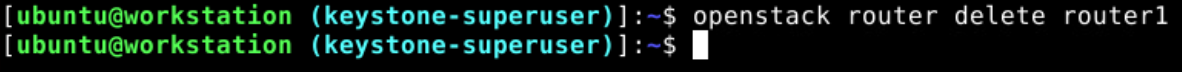
\includegraphics[width=\linewidth]{images/part1/step18.png}
        \end{center}
    \end{labstep}

    \begin{labstep}
        Check that the file created in the previous instance also exists on this instance.
        \begin{lstlisting}
            root@instance1:~# cat /root/hello.txt
        \end{lstlisting}

        \begin{center}
            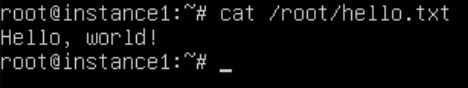
\includegraphics[width=\linewidth]{images/part1/step19.png}
        \end{center}
    \end{labstep}

    \begin{notebox}
        It may take several minutes for the instance to fully boot up and present a login prompt.
    \end{notebox}

    \begin{labstep}
        Exit the instance's console, navigate back to \textbf{Project $>$ Compute $>$ Instances}, and delete the instance.

        \begin{center}
            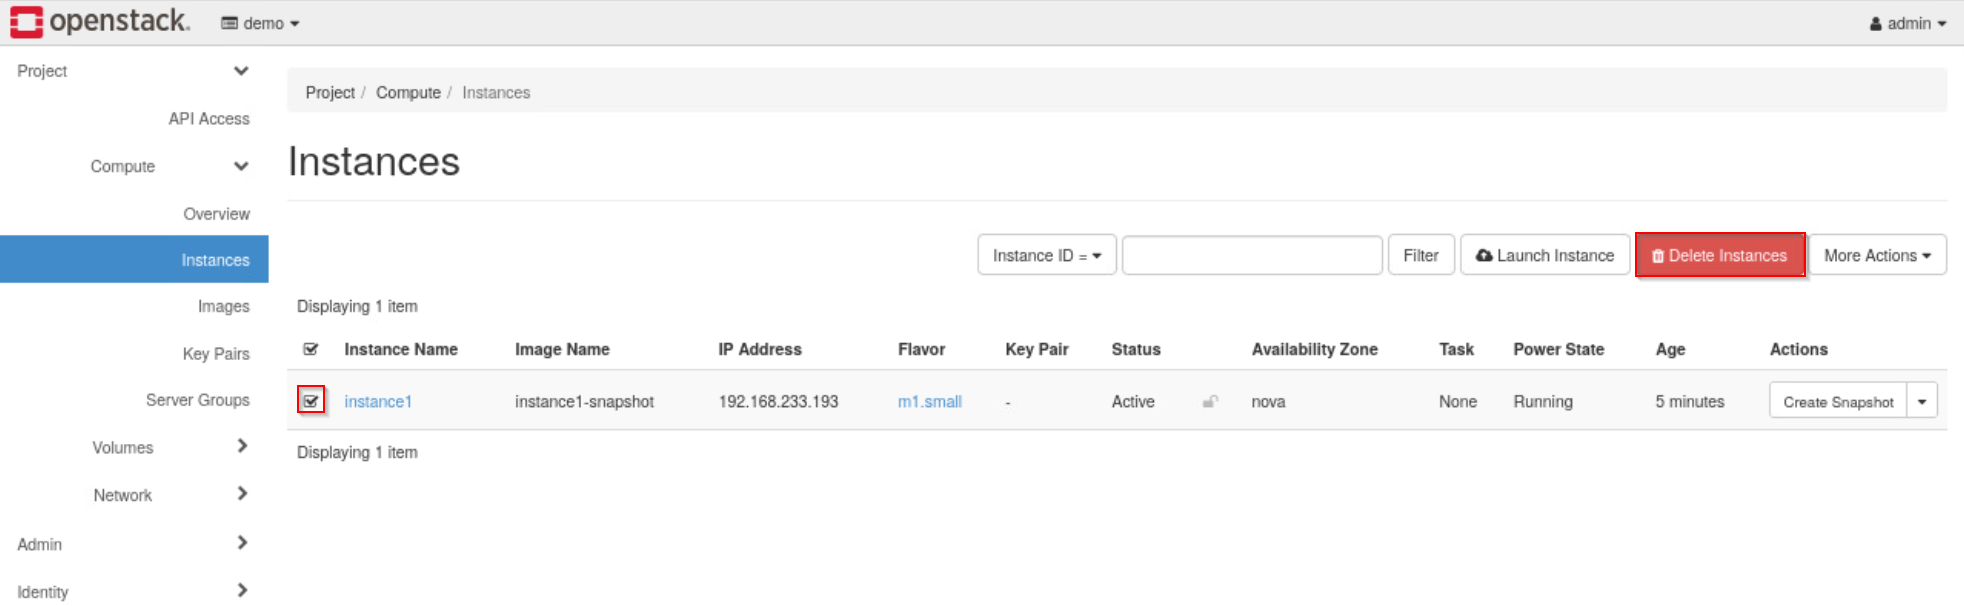
\includegraphics[width=\linewidth]{images/part1/step20.png}
        \end{center}
    \end{labstep}

    \begin{labstep}
        You will create another snapshot with the \textit{OpenStack Unified CLI} in the next task, so \textbf{instance1-snapshot} can safely be deleted.
        Navigate to \textbf{Project $>$ Compute $>$ Images}, select \textbf{instance1-snapshot}, and click \textbf{Delete Images}.

        \begin{center}
            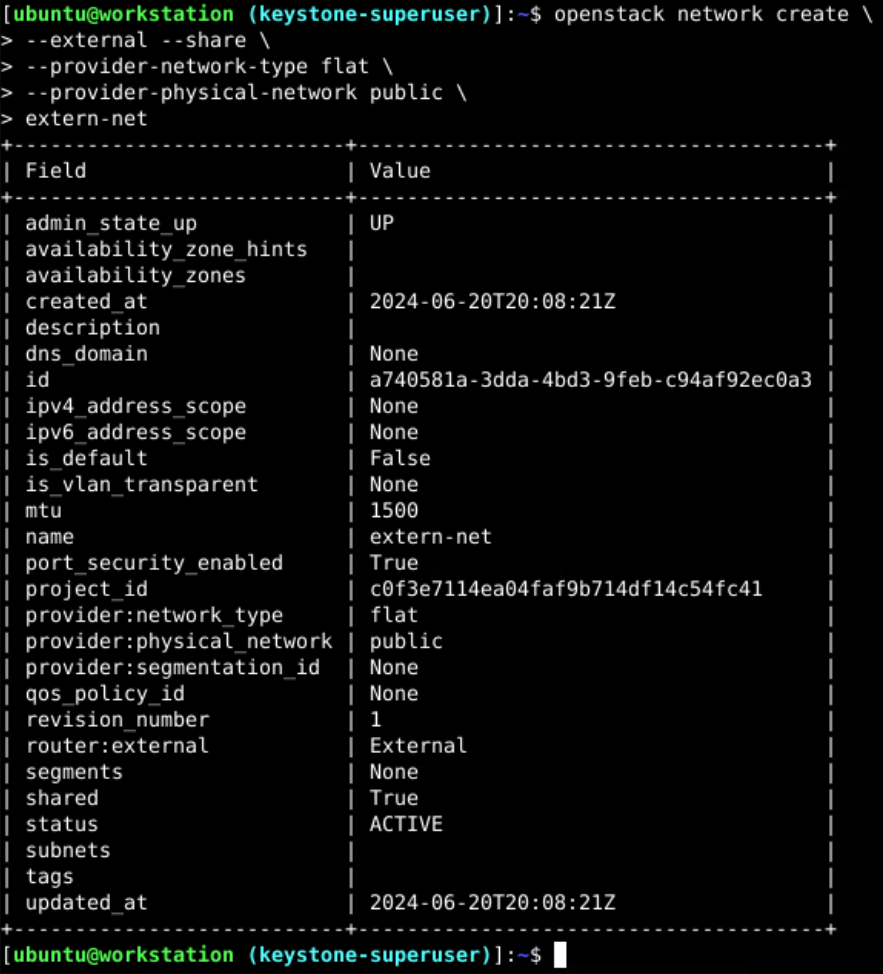
\includegraphics[width=\linewidth]{images/part1/step21.png}
        \end{center}
    \end{labstep}

    \begin{labstep}
        In the \textbf{Confirm Delete Image} dialog, click \textbf{Delete Image}.

        \begin{center}
            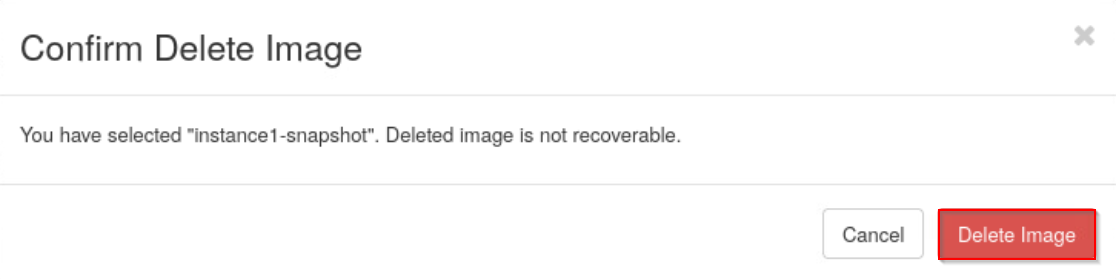
\includegraphics[width=\linewidth]{images/part1/step22.png}
        \end{center}
    \end{labstep}

    \begin{labstep}
        Log out of the dashboard, close the browser window, and continue to the next task.
    \end{labstep}
\end{enumerate}

%%%%%%%%%%%
% Section 2
%%%%%%%%%%%
\section{Creating a Snapshot with the OpenStack Unified CLI}\label{sec:creating-a-snapshot-with-the-openstack-unified-cli}
In this task, you will repeat the steps from the previous task in the \textit{OpenStack Unified CLI}.

\begin{enumerate}
    \begin{labstep}
        Open a terminal window and source the keystone credentials for the \textbf{admin} user.
        \begin{lstlisting}
            ubuntu@workstation:~$ source ~/keystonerc-admin
        \end{lstlisting}

        \begin{center}
            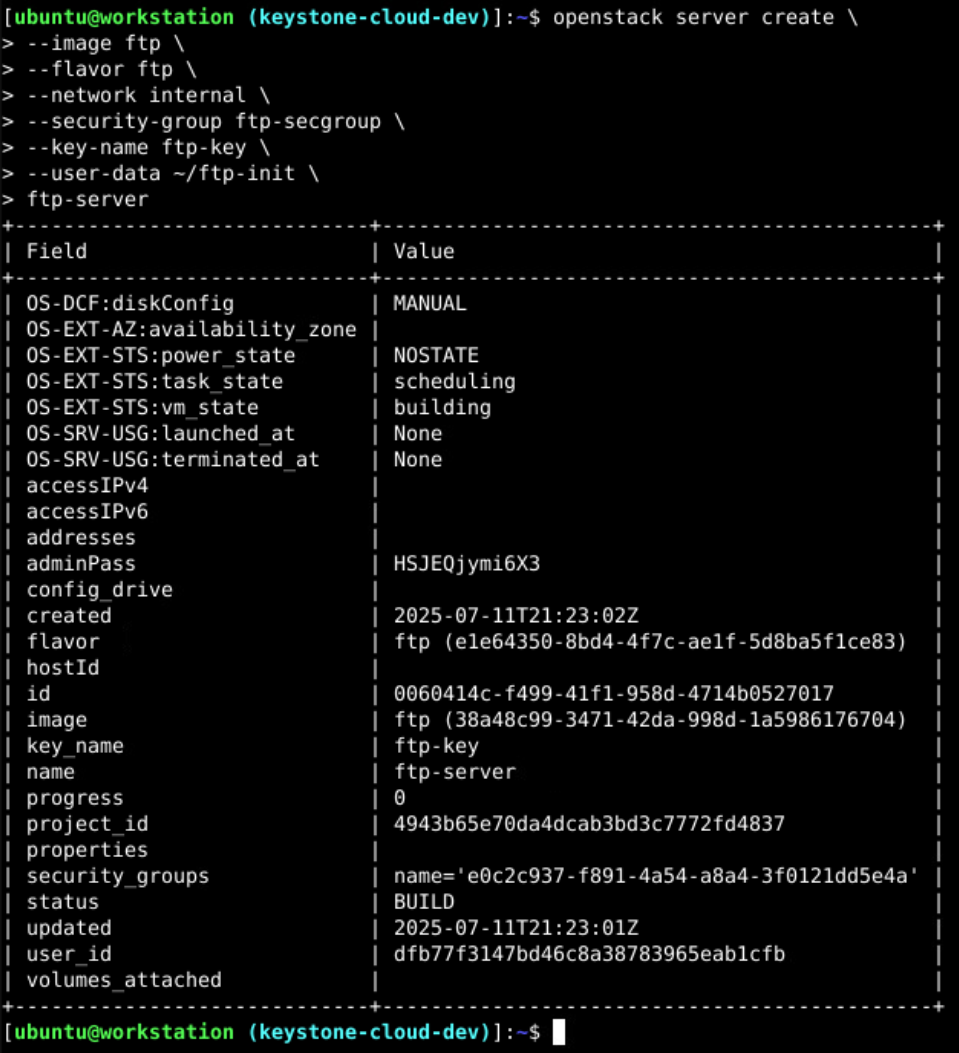
\includegraphics[width=\linewidth]{images/part2/step1.png}
        \end{center}
    \end{labstep}

    \begin{labstep}
        List the current instances.
        The list should be empty.
        \begin{lstlisting}
            [ubuntu@workstation (keystone-admin)]:~$ openstack server list
        \end{lstlisting}

        \begin{center}
            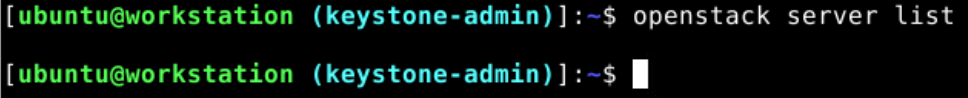
\includegraphics[width=\linewidth]{images/part2/step2.png}
        \end{center}
    \end{labstep}

    \begin{labstep}
        Now, we will create the same snapshot as before from the command line.
        Launch an instance.
        Use the \textbf{ubuntu} image, the \textbf{m1.small} flavor, and the \textbf{shared} network.
        \begin{lstlisting}
            [ubuntu@workstation (keystone-admin)]:~$ openstack server create \
            > --image ubuntu \
            > --flavor m1.small \
            > --network shared \
            instance2
        \end{lstlisting}

        \begin{center}
            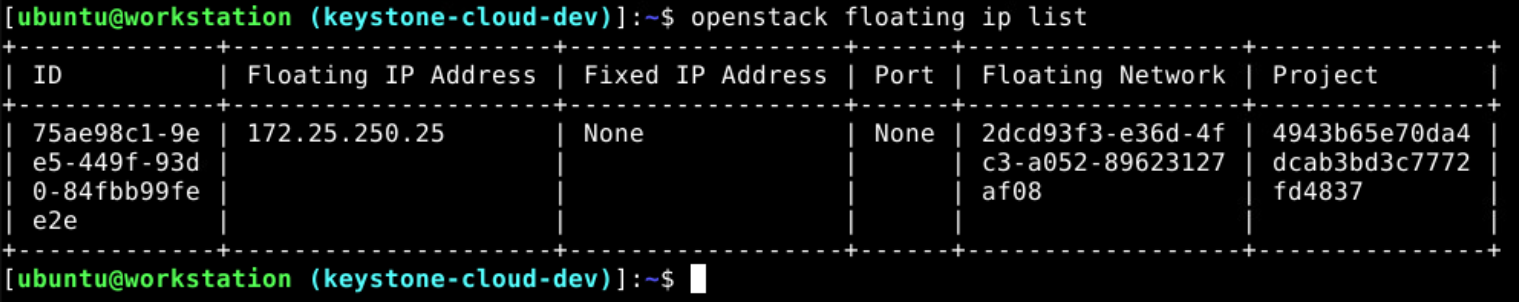
\includegraphics[width=\linewidth]{images/part2/step3.png}
        \end{center}
    \end{labstep}

    \begin{labstep}
        List the instances again to ensure it was created correctly.
        \begin{lstlisting}
            [ubuntu@workstation (keystone-admin)]:~$ openstack server list
        \end{lstlisting}

        \begin{center}
            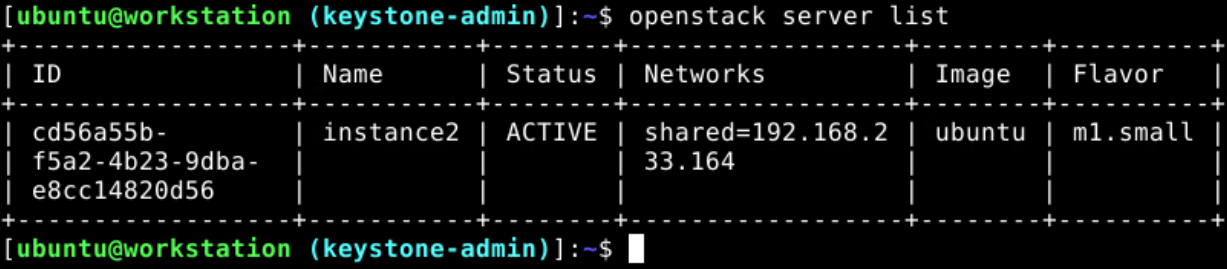
\includegraphics[width=\linewidth]{images/part2/step4.png}
        \end{center}
    \end{labstep}

    \begin{tipbox}
        When typing the command, make sure there is a space between \textbf{list} and the \textbf{\textbackslash} character, and press \textbf{Enter} to get the \textbf{$>$} and continue typing the rest of the command.
    \end{tipbox}

    \begin{labstep}
        Show the URL to the console of the instance.
        Right-click the URL and click \textbf{Open Link}.
        \begin{lstlisting}
            [ubuntu@workstation (keystone-admin)]:~$ openstack console url show instance2
        \end{lstlisting}

        \begin{center}
            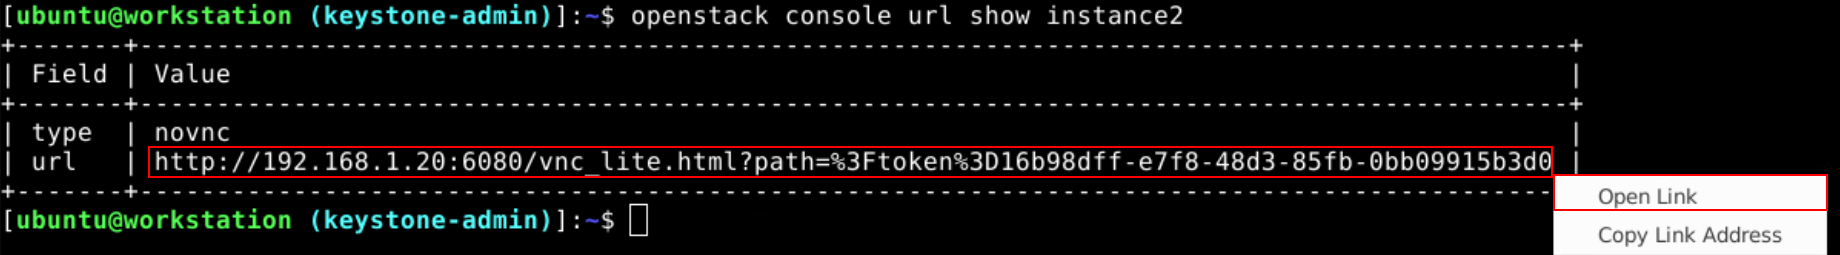
\includegraphics[width=\linewidth]{images/part2/step5.png}
        \end{center}
    \end{labstep}

    \begin{labstep}
        Log in to \textbf{instance2} as \textbf{root} with the password \textbf{secret}.

        \begin{center}
            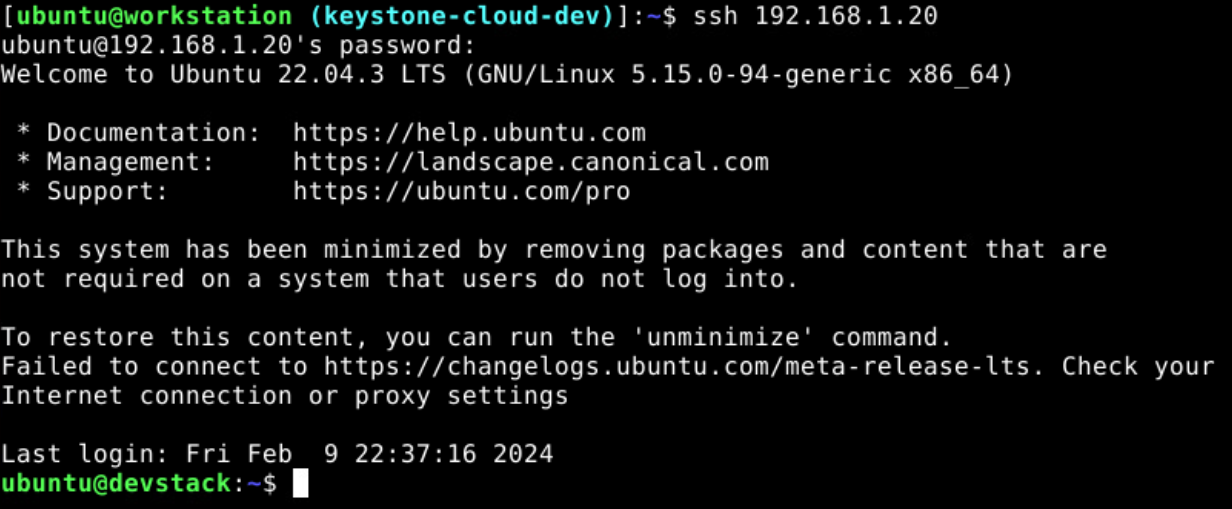
\includegraphics[width=\linewidth]{images/part2/step6.png}
        \end{center}
    \end{labstep}

    \begin{notebox}
        It may take several minutes for the instance to fully boot up and present a login prompt.
    \end{notebox}

    \begin{labstep}
        Create the \textbf{/root/hello.txt} file with the contents \textbf{Hello, world!}.
        \begin{lstlisting}
            root@instance2:~# echo 'Hello, world!' > /root/hello.txt
        \end{lstlisting}

        \begin{center}
            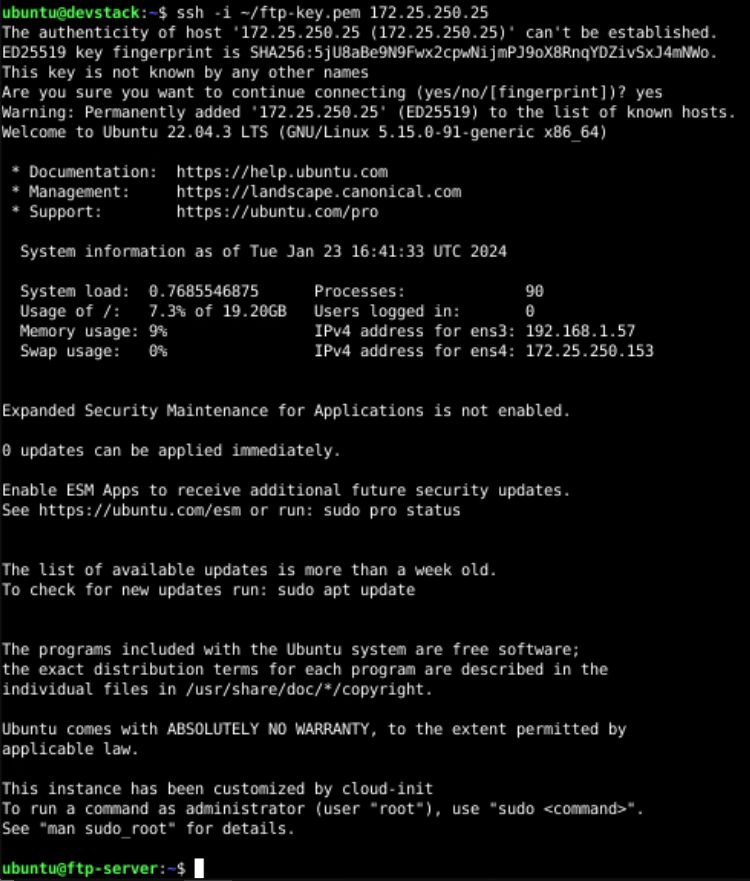
\includegraphics[width=\linewidth]{images/part2/step7.png}
        \end{center}
    \end{labstep}

    \begin{labstep}
        Close the browser window and return focus to the terminal window.
        Stop the instance before making a snapshot.
        \begin{lstlisting}
            [ubuntu@workstation (keystone-admin)]:~$ openstack server stop instance2
        \end{lstlisting}

        \begin{center}
            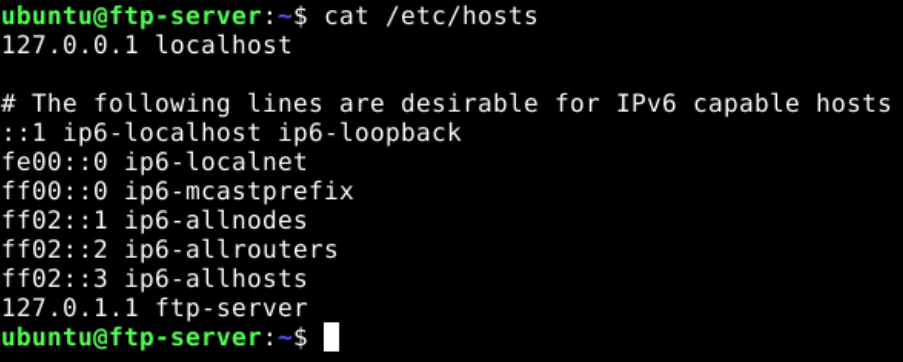
\includegraphics[width=\linewidth]{images/part2/step8.png}
        \end{center}
    \end{labstep}

    \begin{labstep}
        List the current images.
        The list should have two items.
        \begin{lstlisting}
            [ubuntu@workstation (keystone-admin)]:~$ openstack image list
        \end{lstlisting}

        \begin{center}
            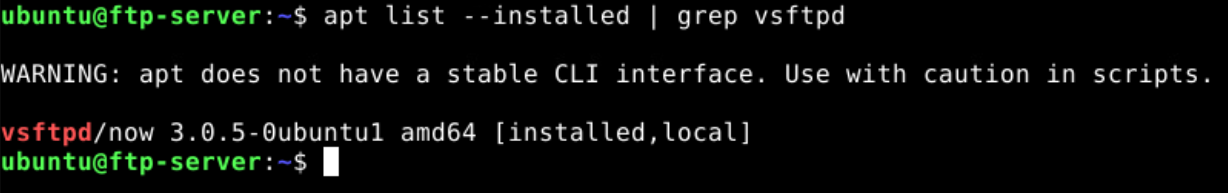
\includegraphics[width=\linewidth]{images/part2/step9.png}
        \end{center}
    \end{labstep}

    \begin{labstep}
        Make a snapshot of the instance.
        \begin{lstlisting}
            [ubuntu@workstation (keystone-admin)]:~$ openstack server image create \
            > --name instance2-snapshot \
            > instance2
        \end{lstlisting}

        \begin{center}
            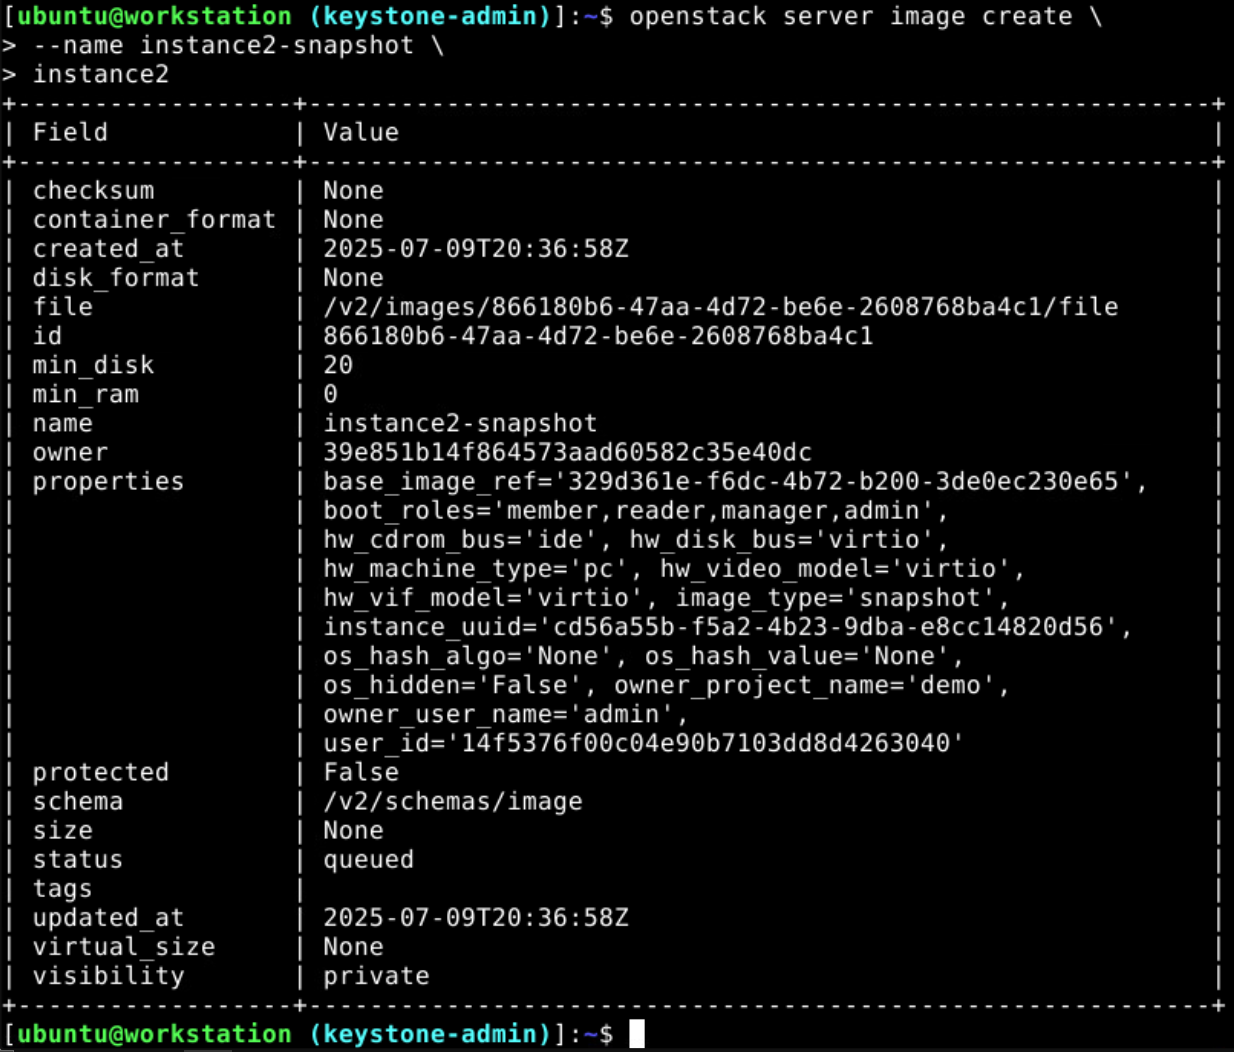
\includegraphics[width=\linewidth]{images/part2/step10.png}
        \end{center}
    \end{labstep}

    \begin{labstep}
        List the current images again to ensure the snapshot was created properly.
        \begin{lstlisting}
            [ubuntu@workstation (keystone-admin)]:~$ openstack image list
        \end{lstlisting}

        \begin{center}
            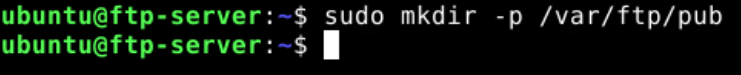
\includegraphics[width=\linewidth]{images/part2/step11.png}
        \end{center}
    \end{labstep}

    \begin{labstep}
        To verify the correctness of the snapshot, first delete the instance.
        \begin{lstlisting}
            [ubuntu@workstation (keystone-admin)]:~$ openstack server delete instance2
        \end{lstlisting}

        \begin{center}
            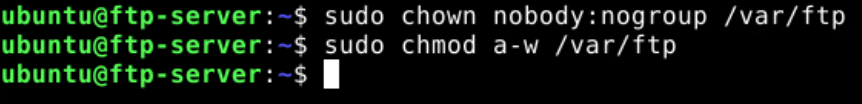
\includegraphics[width=\linewidth]{images/part2/step12.png}
        \end{center}
    \end{labstep}

    \begin{labstep}
        Confirm the deletion of the instance.
        \begin{lstlisting}
            [ubuntu@workstation (keystone-admin)]:~$ openstack server list
        \end{lstlisting}

        \begin{center}
            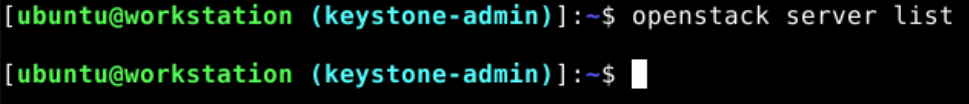
\includegraphics[width=\linewidth]{images/part2/step13.png}
        \end{center}
    \end{labstep}

    \begin{labstep}
        Now, recreate the instance, using \textbf{instance2-snapshot} as the image.
        \begin{lstlisting}
            [ubuntu@workstation (keystone-admin)]:~$ openstack server create \
            > --image instance2-snapshot \
            > --flavor m1.small \
            > --network shared \
            instance2
        \end{lstlisting}

        \begin{center}
            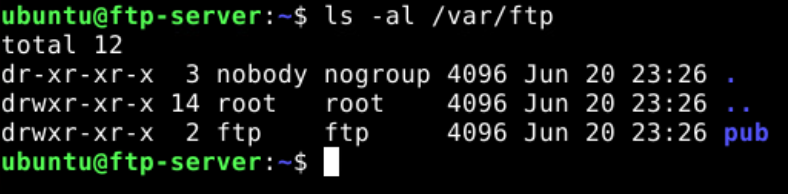
\includegraphics[width=\linewidth]{images/part2/step14.png}
        \end{center}
    \end{labstep}

    \begin{labstep}
        Using the same steps as before, log in to the instance's console as \textbf{root} with the password \textbf{secret}.

        \begin{center}
            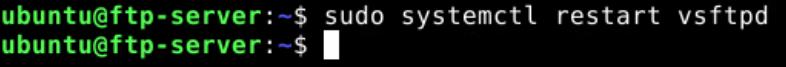
\includegraphics[width=\linewidth]{images/part2/step15.png}
        \end{center}
    \end{labstep}

    \begin{notebox}
        It may take several minutes for the instance to fully boot up and present a login prompt.
    \end{notebox}

    \begin{labstep}
        Verify that the \textbf{/root/hello.txt} file exists.
        \begin{lstlisting}
            root@instance2:~# cat /root/hello.txt
        \end{lstlisting}

        \begin{center}
            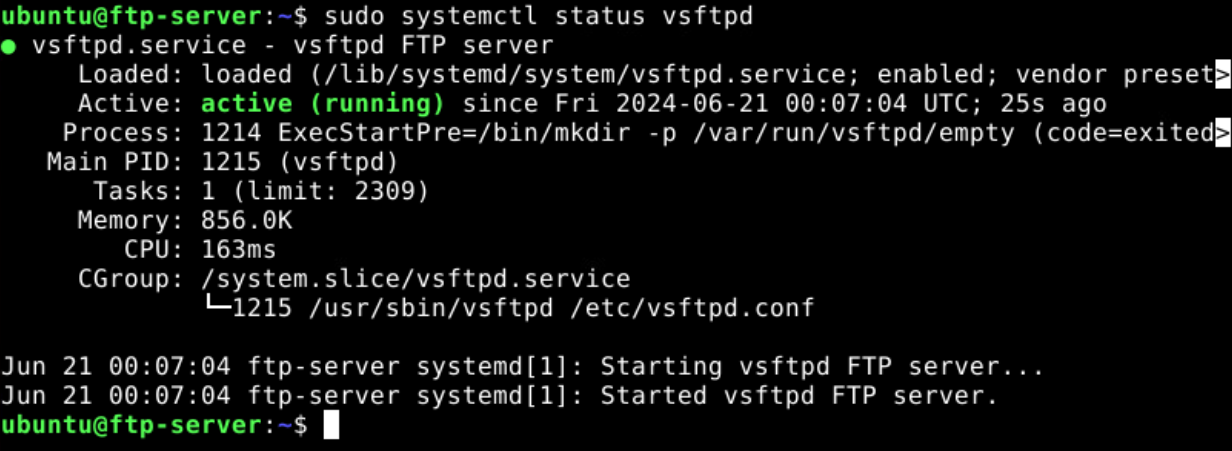
\includegraphics[width=\linewidth]{images/part2/step16.png}
        \end{center}
    \end{labstep}

    \begin{labstep}
        Close the browser window, and delete the instance.
        \begin{lstlisting}
            [ubuntu@workstation (keystone-admin)]:~$ openstack server delete instance2
        \end{lstlisting}

        \begin{center}
            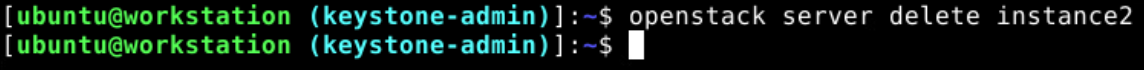
\includegraphics[width=\linewidth]{images/part2/step17.png}
        \end{center}
    \end{labstep}

    \begin{labstep}
        Delete the \textbf{instance2-snapshot} image.
        \begin{lstlisting}
            [ubuntu@workstation (keystone-admin)]:~$ openstack image delete \
            > instance2-snapshot
        \end{lstlisting}

        \begin{center}
            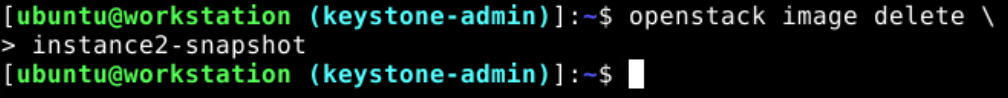
\includegraphics[width=\linewidth]{images/part2/step18.png}
        \end{center}
    \end{labstep}

    \begin{labstep}
        Leave the terminal window open, and continue to the next task.
    \end{labstep}

\end{enumerate}

%%%%%%%%%%%
% Section 3
%%%%%%%%%%%
\section{Managing the Running State of an Instance with the Horizon Dashboard}\label{sec:managing-the-running-state-of-an-instance-with-the-horizon-dashboard}
OpenStack allows for managing the running and power state of instances in a variety of ways, and each method is useful in different situations.
In this task, you will manage the running and power state of an instance by starting, stopping, pausing, suspending, resuming, and rebooting the instance with the \textit{Horizon Dashboard}.

\begin{enumerate}
    \begin{labstep}
        If a terminal window is not already open, open one and source the keystone credentials for the \textbf{admin} user.
        \begin{lstlisting}
            ubuntu@workstation:~$ source ~/keystonerc-admin
        \end{lstlisting}

        \begin{center}
            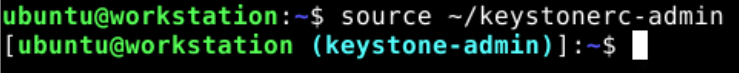
\includegraphics[width=\linewidth]{images/part3/step1.png}
        \end{center}
    \end{labstep}

    \begin{labstep}
        Create an instance named \textbf{instance3}.
        Use the \textbf{ubuntu} image and the \textbf{m1.small} flavor, and connect the instance to the \textbf{shared} network.
        \begin{lstlisting}
            [ubuntu@workstation (keystone-admin)]:~$ openstack server create \
            > --image ubuntu \
            > --flavor m1.small \
            > --network shared \
            instance3
        \end{lstlisting}

        \begin{center}
            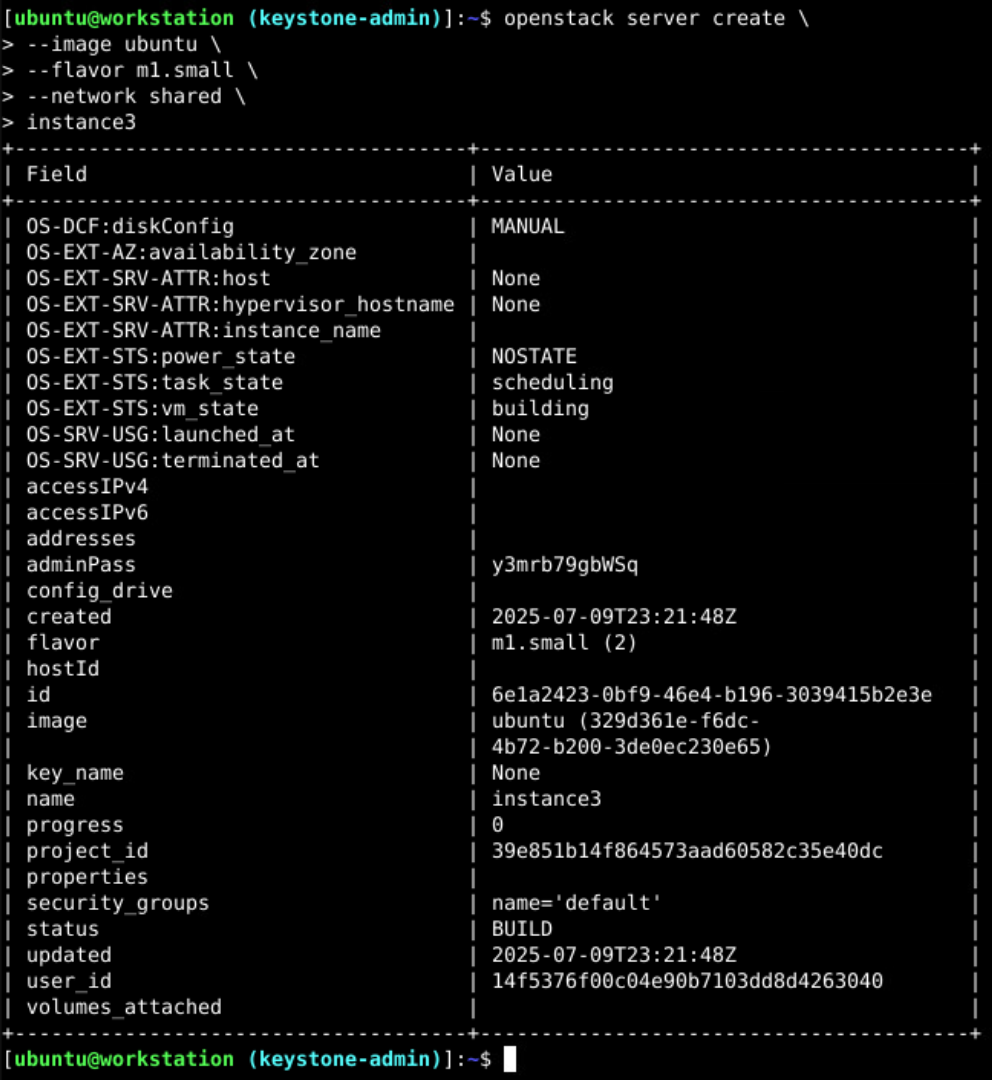
\includegraphics[width=\linewidth]{images/part3/step2.png}
        \end{center}
    \end{labstep}

    \begin{labstep}
        Close the terminal window.
        Open a browser window, and navigate to \textbf{192.168.1.20}.
        Log in as \textbf{admin} with the password \textbf{secret}.

        \begin{center}
            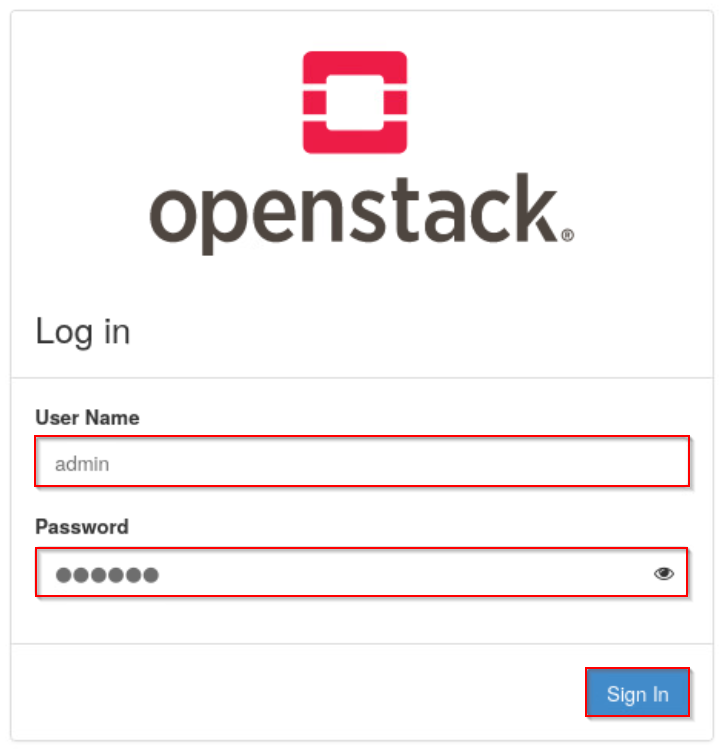
\includegraphics[scale=0.5]{images/part3/step3.png}
        \end{center}
    \end{labstep}

    \begin{labstep}
        Navigate to \textbf{Project $>$ Compute $>$ Instances}.
        Open the \textbf{instance3} link in a new tab.

        \begin{center}
            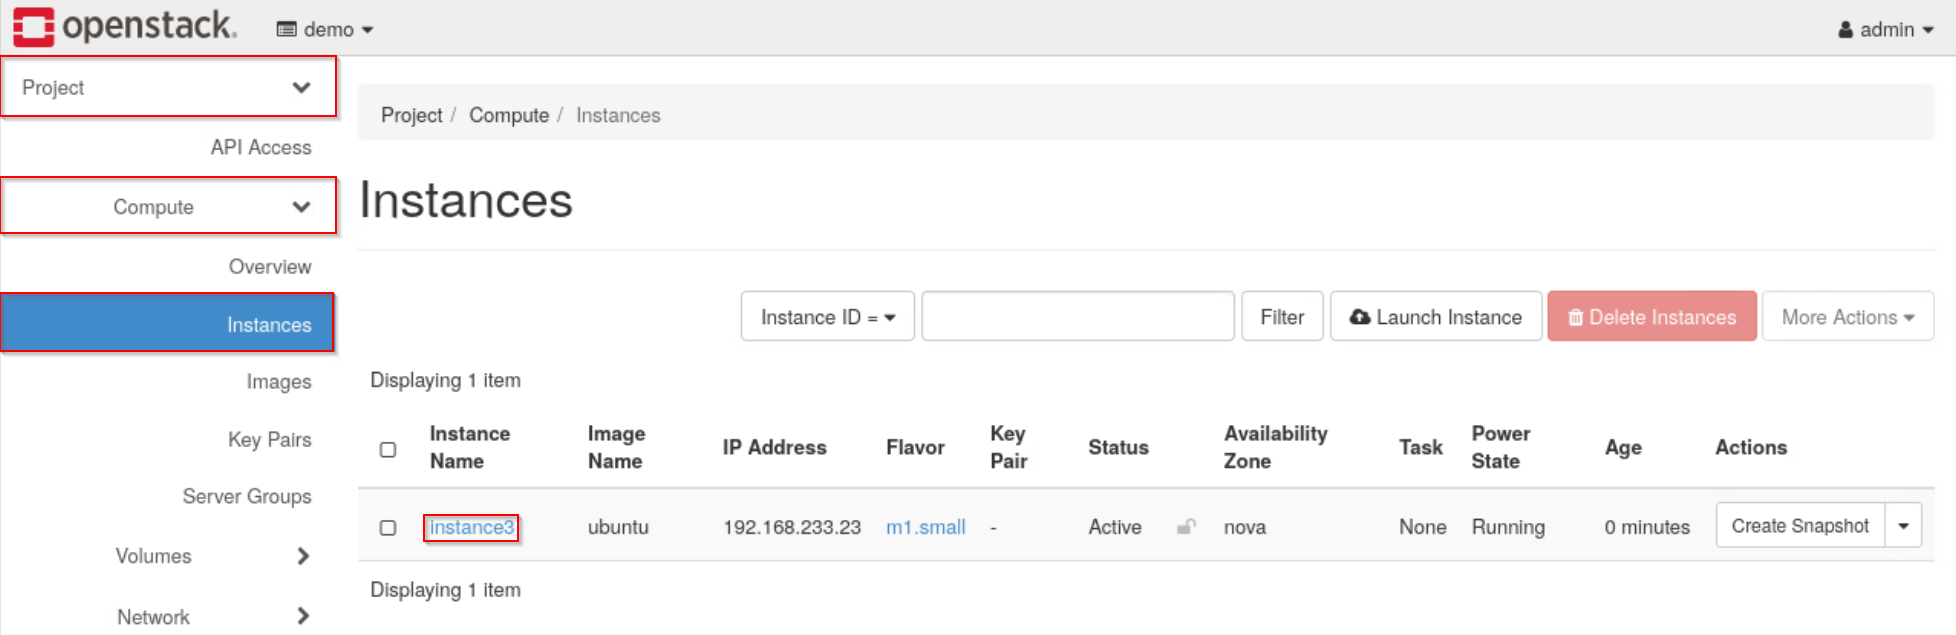
\includegraphics[width=\linewidth]{images/part3/step4.png}
        \end{center}
    \end{labstep}

    \begin{labstep}
        Navigate to the \textit{Console} tab, and click the \textbf{Click here to show only console} link.

        \begin{center}
            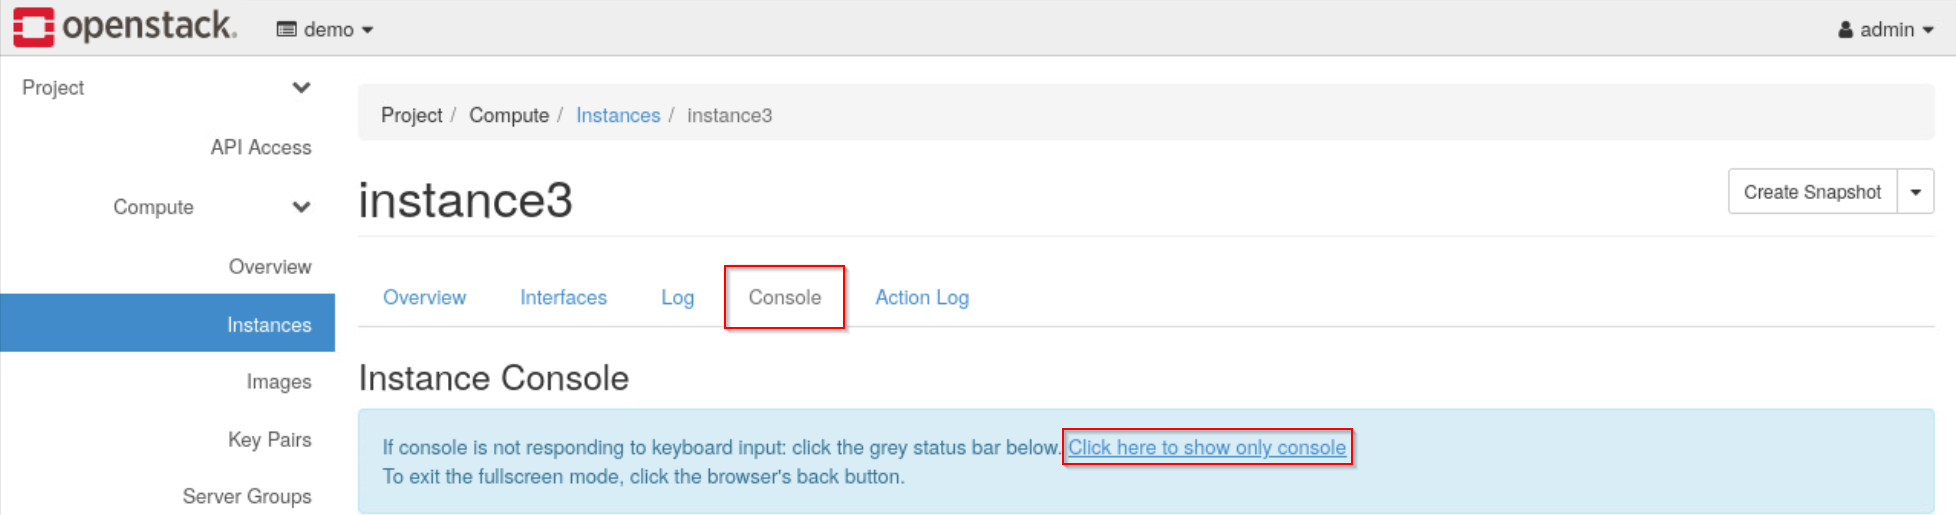
\includegraphics[width=\linewidth]{images/part3/step5.png}
        \end{center}
    \end{labstep}

    \begin{labstep}
        Log in as \textbf{root} with the password \textbf{secret}.

        \begin{center}
            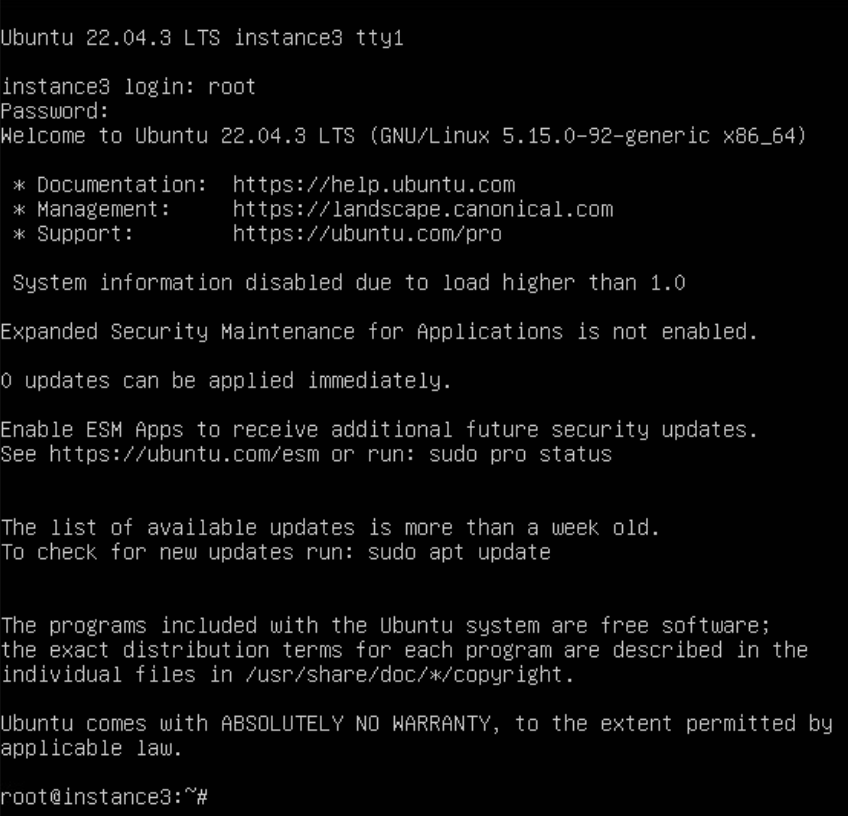
\includegraphics[width=\linewidth]{images/part3/step6.png}
        \end{center}
    \end{labstep}

    \begin{notebox}
        It may take several minutes for the instance to fully boot up and present a login prompt.
    \end{notebox}

    \begin{labstep}
        Pausing an instance is one way to manage the running state of an OpenStack instance.
        When an instance is paused, its operation is frozen, and its state and memory are preserved in the RAM of the underlying compute node.
        Pausing an instance does not release its resources.
        When the instance is resumed, it will pick up any processes where they left off.
        To view the effects of pausing an instance, first start continuously pinging the DHCP server.
        \begin{lstlisting}
            root@instance3:~# ping 192.168.233.2
        \end{lstlisting}

        \begin{center}
            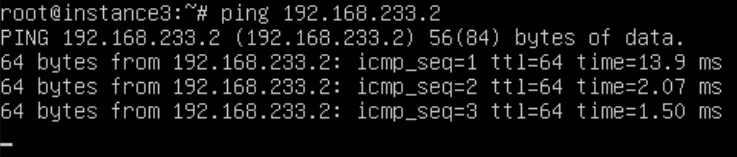
\includegraphics[width=\linewidth]{images/part3/step7.png}
        \end{center}
    \end{labstep}

    \begin{tipbox}
        Pausing an instance is useful when the operation of an instance needs to be interrupted while its state should be kept intact.
        For example, an instance might be paused while making changes to the underlying infrastructure to prevent disrupting processes and requiring applications or the instance to be restarted.
        Pausing an instance is similar to putting a computer in sleep mode.
    \end{tipbox}

    \begin{labstep}
        To pause the instance, navigate to \textbf{Project $>$ Compute $>$ Instances}, click the dropdown next to \textbf{Create Snapshot} in the same row as \textbf{instance3}, scroll down if necessary, and click \textbf{Pause Instance}.

        \begin{center}
            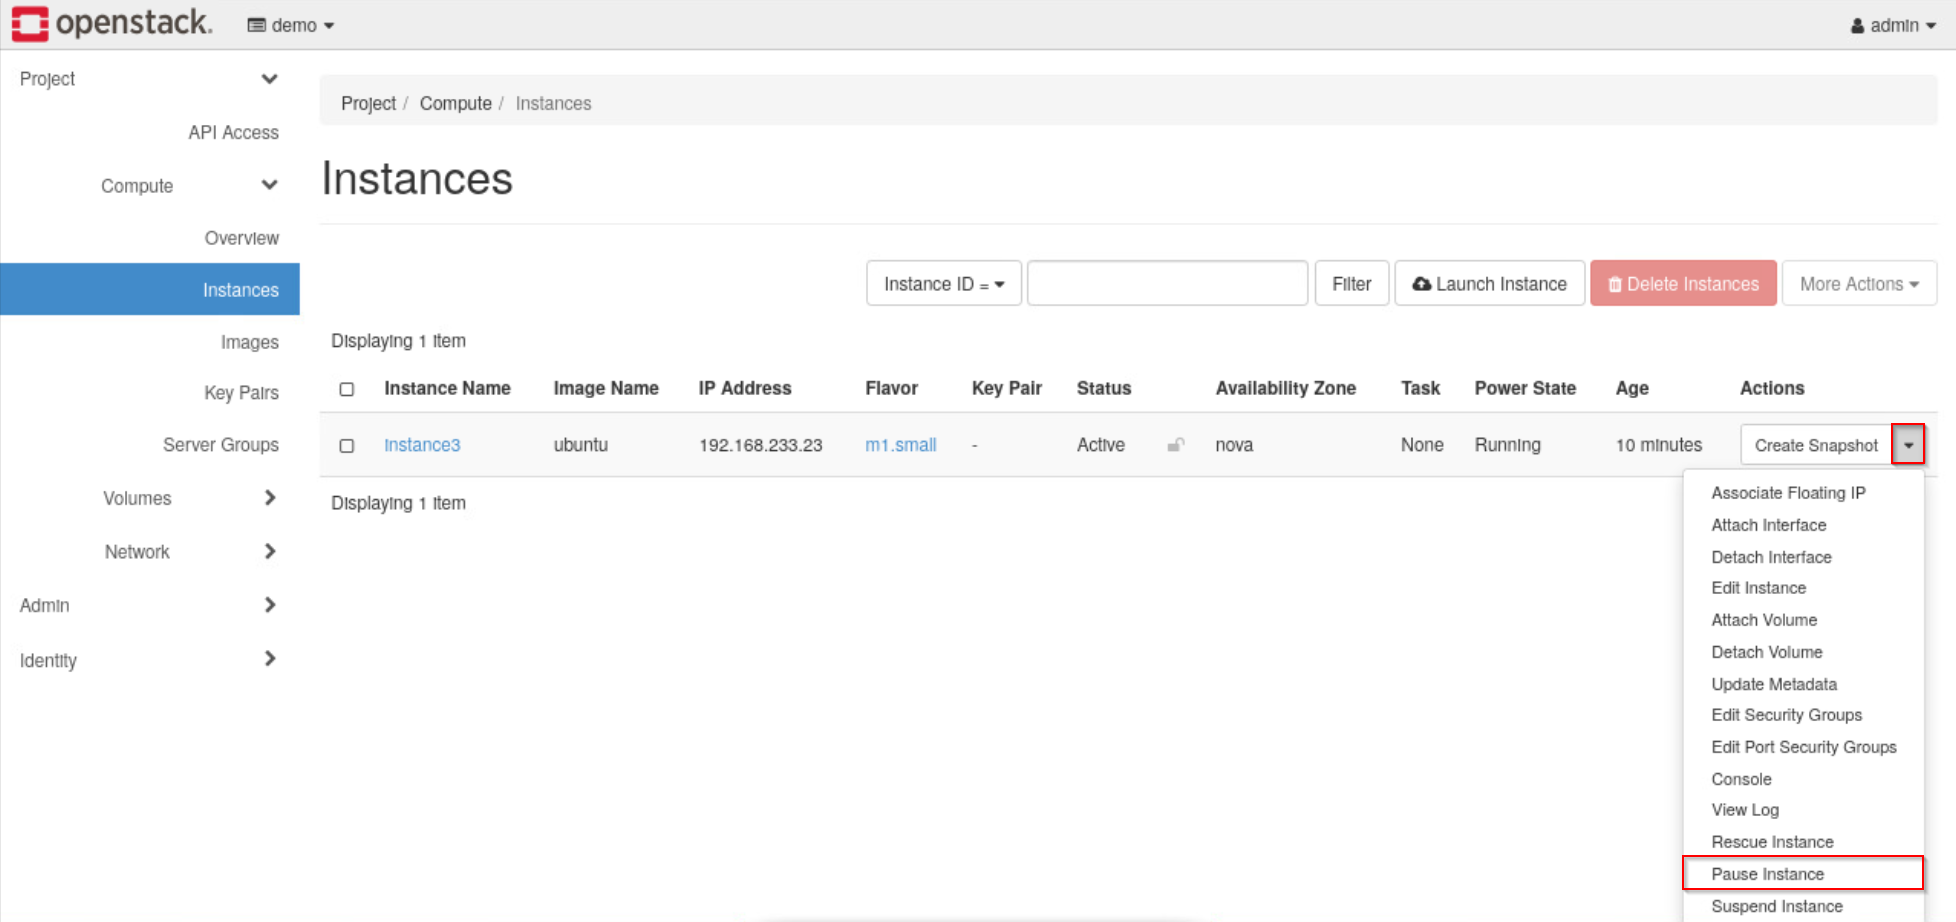
\includegraphics[width=\linewidth]{images/part3/step8.png}
        \end{center}
    \end{labstep}

    \begin{stopbox}
        Wait until the instance's status becomes \textbf{Paused}.
    \end{stopbox}

    \begin{labstep}
        Now, view the console again to see that it is frozen and no more ping replies are appearing.

        \begin{center}
            \includegraphics[width=\linewidth]{images/part3/step9.png}
        \end{center}
    \end{labstep}

    \begin{labstep}
        Navigate back to the \textbf{Instances} page.
        Click the dropdown next to \textbf{Create Snapshot} in the same row as \textbf{instance2} and click \textbf{Resume Instance}.

        \begin{center}
            \includegraphics[width=\linewidth]{images/part3/step10.png}
        \end{center}
    \end{labstep}

    \begin{stopbox}
        Wait until the instance's status becomes \textbf{Active}.
    \end{stopbox}

    \begin{labstep}
        View the console again to see that the ping replies have resumed.
        Press \textbf{Ctrl+C} to stop the \textbf{ping} command.

        \begin{center}
            \includegraphics[width=\linewidth]{images/part3/step11.png}
        \end{center}
    \end{labstep}

    \begin{labstep}
        Suspending an instance is similar to pausing an instance.
        The main difference is that the instance's state is written to a persistent disk of the underlying compute node rather than memory.
        This means the state can be preserved even if the compute node loses power during the suspension.
        Suspending an instance does not release its resources.
        When the instance is resumed, it will pick up any processes where they left off.
        To view the effects of suspending an instance, perform the same experiment as before.
        Focus on the tab with the instance's console and continuously ping the DHCP server.
        \begin{lstlisting}
            root@instance3:~# ping 192.168.233.2
        \end{lstlisting}

        \begin{center}
            \includegraphics[width=\linewidth]{images/part3/step12.png}
        \end{center}
    \end{labstep}

    \begin{tipbox}
        Suspending an instance is useful in similar situations as pausing.
        However, suspending an image allows the compute node to be rebooted or migrated without disrupting the processes of the instance and requiring applications or the instance to be restarted.
        Suspending an instance is similar to putting a computer in hibernation mode.
    \end{tipbox}

    \begin{labstep}
        To suspend the instance, navigate back to \textbf{Project $>$ Compute $>$ Instances}, click the dropdown next to \textbf{Create Snapshot}, scroll down if necessary, and click \textbf{Suspend Instance}.

        \begin{center}
            \includegraphics[width=\linewidth]{images/part3/step13.png}
        \end{center}
    \end{labstep}

    \begin{stopbox}
        Wait until the instance's status becomes \textbf{Suspended}.
    \end{stopbox}

    \begin{labstep}
        View the console again to see that the connection has been ended.
        When the instance is resumed, a new connection will be created, and this tab will still be unresponsive.
        Close the tab containing the instance console.

        \begin{center}
            \includegraphics[width=\linewidth]{images/part3/step14.png}
        \end{center}
    \end{labstep}

    \begin{labstep}
        Navigate back to the \textbf{Instances} page.
        Click the dropdown next to \textbf{Create Snapshot} in the same row as \textbf{instance3} and click \textbf{Resume Instance}.

        \begin{center}
            \includegraphics[width=\linewidth]{images/part3/step15.png}
        \end{center}
    \end{labstep}

    \begin{stopbox}
        Wait until the instance's status becomes \textbf{Active}.
    \end{stopbox}

    \begin{labstep}
        Click \textbf{instance3} and select the \textbf{Console} tab to see that the ping replies have resumed.
        Press \textbf{Ctrl+C} to stop the \textbf{ping} process.

        \begin{center}
            \includegraphics[width=\linewidth]{images/part3/step16.png}
        \end{center}
    \end{labstep}

    \begin{labstep}
        Shutting off or stopping an instance turns off the instance.
        The instance state and any data stored in the instance's RAM will be lost.
        Stopping an instance does not release its resources.
        To stop an instance, navigate to the \textbf{Instances} page.
        Click the dropdown next to \textbf{Create Snapshot} in the same row as \textbf{instance3}, scroll down if necessary, and click \textbf{Shut Off Instance}.

        \begin{center}
            \includegraphics[width=\linewidth]{images/part3/step17.png}
        \end{center}
    \end{labstep}

    \begin{stopbox}
        Wait until the instance's status becomes \textbf{Shutoff}.
    \end{stopbox}

    \begin{labstep}
        In the \textbf{Confirm Shut Off Instance} dialog, click \textbf{Shut Off Instance}.

        \begin{center}
            \includegraphics[width=\linewidth]{images/part3/step18.png}
        \end{center}
    \end{labstep}

    \begin{labstep}
        When the power state of the instance indicates that it is shut off, the \textbf{Create Snapshot} button will become \textbf{Start Instance}.
        Click this button to turn the instance back on.

        \begin{center}
            \includegraphics[width=\linewidth]{images/part3/step19.png}
        \end{center}
    \end{labstep}

    \begin{stopbox}
        Wait until the instance's status becomes \textbf{Active}.
    \end{stopbox}
    \begin{tipbox}
        In addition to shutting off an instance, an instance can also be soft or hard rebooted, or turned off and back on.
        A soft reboot allows the instance to perform a graceful shutdown, while hard rebooting an instance is analogous to pulling the power cord from a computer.
    \end{tipbox}

    \begin{labstep}
        Close the browser window, and continue to the next task.
    \end{labstep}

\end{enumerate}

%%%%%%%%%%%
% Section 4
%%%%%%%%%%%
\section{Managing the Running State of an Instance with the OpenStack Unified CLI}\label{sec:managing-the-power-state-of-an-instance-with-the-openstack-unified-cli}
In this task, you will repeat the steps from the previous task in the \textit{OpenStack Unified CLI}.

\begin{enumerate}
    \begin{labstep}
        Open a terminal window, and source the keystone credentials for the \textbf{admin} user.
        \begin{lstlisting}
            ubuntu@workstation:~$ source ~/keystonerc-admin
        \end{lstlisting}

        \begin{center}
            \includegraphics[width=\linewidth]{images/part4/step1.png}
        \end{center}
    \end{labstep}

    \begin{labstep}
        Maximize the terminal window.
        Show the URL to the console of the instance.
        Right-click the URL and click \textbf{Open Link}.
        \begin{lstlisting}
            [ubuntu@workstation (keystone-admin)]:~$ openstack console url show instance3
        \end{lstlisting}

        \begin{center}
            \includegraphics[width=\linewidth]{images/part4/step2.png}
        \end{center}
    \end{labstep}

    \begin{tipbox}
        If the URL is split over multiple lines, you will not be able to follow the link.
    \end{tipbox}

    \begin{labstep}
        Log in to \textbf{instance3} as \textbf{root} with the password \textbf{secret}.

        \begin{center}
            \includegraphics[width=\linewidth]{images/part4/step3.png}
        \end{center}
    \end{labstep}

    \begin{labstep}
        Continuously ping the DHCP server to see the effects of pausing an instance.
        \begin{lstlisting}
            root@instance3:~# ping 192.168.233.2
        \end{lstlisting}

        \begin{center}
            \includegraphics[width=\linewidth]{images/part4/step4.png}
        \end{center}
    \end{labstep}

    \begin{labstep}
        Focus back on the terminal window and pause the instance.
        \begin{lstlisting}
            [ubuntu@workstation (keystone-admin)]:~$ openstack server pause instance3
        \end{lstlisting}

        \begin{center}
            \includegraphics[width=\linewidth]{images/part4/step5.png}
        \end{center}
    \end{labstep}

    \begin{labstep}
        Now, view the browser window again to see that the instance is frozen and no more ping replies are appearing.

        \begin{center}
            \includegraphics[width=\linewidth]{images/part4/step6.png}
        \end{center}
    \end{labstep}

    \begin{labstep}
        Focus back on the terminal window and resume the instance
        \begin{lstlisting}
            [ubuntu@workstation (keystone-admin)]:~$ openstack server unpause instance3
        \end{lstlisting}

        \begin{center}
            \includegraphics[width=\linewidth]{images/part4/step7.png}
        \end{center}
    \end{labstep}

    \begin{labstep}
        View the browser window again to see that more ping replies are coming in.
        Press \textbf{Ctrl+C} to stop the \textbf{ping} process.

        \begin{center}
            \includegraphics[width=\linewidth]{images/part4/step8.png}
        \end{center}
    \end{labstep}

    \begin{labstep}
        Start the \textbf{ping} process again to view the effects of suspending an instance.
        \begin{lstlisting}
            root@instance3:~# ping 192.168.233.2
        \end{lstlisting}

        \begin{center}
            \includegraphics[width=\linewidth]{images/part4/step9.png}
        \end{center}
    \end{labstep}

    \begin{labstep}
        Focus back on the terminal window and suspend the instance.
        \begin{lstlisting}
            [ubuntu@workstation (keystone-admin)]:~$ openstack server suspend instance3
        \end{lstlisting}

        \begin{center}
            \includegraphics[width=\linewidth]{images/part4/step10.png}
        \end{center}
    \end{labstep}

    \begin{labstep}
        View the console again to see that the connection has been ended.
        When the instance is resumed, a new connection will be created, and this tab will still be unresponsive.
        Close the browser window.

        \begin{center}
            \includegraphics[width=\linewidth]{images/part4/step11.png}
        \end{center}
    \end{labstep}

    \begin{labstep}
        Focus back on the terminal window and resume the instance.
        \begin{lstlisting}
            [ubuntu@workstation (keystone-admin)]:~$ openstack server resume instance3
        \end{lstlisting}

        \begin{center}
            \includegraphics[width=\linewidth]{images/part4/step12.png}
        \end{center}
    \end{labstep}

    \begin{labstep}
        Show the URL to the console of the instance.
        Right-click the URL and click \textbf{Open Link}.
        \begin{lstlisting}
            [ubuntu@workstation (keystone-admin)]:~$ openstack console url show instance3
        \end{lstlisting}

        \begin{center}
            \includegraphics[width=\linewidth]{images/part4/step13.png}
        \end{center}
    \end{labstep}

    \begin{labstep}
        Log in to \textbf{instance3} as \textbf{root} with the password \textbf{secret}.

        \begin{center}
            \includegraphics[width=\linewidth]{images/part4/step14.png}
        \end{center}
    \end{labstep}

    \begin{labstep}
        Note that more ping replies are now coming in.
        Press \textbf{Ctrl+C} to stop the \textbf{ping} command, and close the browser window.

        \begin{center}
            \includegraphics[width=\linewidth]{images/part4/step15.png}
        \end{center}
    \end{labstep}

    \begin{labstep}
        Focus back on the terminal window and confirm that \textbf{instance3} is listed as \textbf{ACTIVE}.
        \begin{lstlisting}
            [ubuntu@workstation (keystone-admin)]:~$ openstack server list
        \end{lstlisting}

        \begin{center}
            \includegraphics[width=\linewidth]{images/part4/step16.png}
        \end{center}
    \end{labstep}

    \begin{labstep}
        Stop the instance.
        \begin{lstlisting}
            [ubuntu@workstation (keystone-admin)]:~$ openstack server stop instance3
        \end{lstlisting}

        \begin{center}
            \includegraphics[width=\linewidth]{images/part4/step17.png}
        \end{center}
    \end{labstep}

    \begin{labstep}
        Verify that the status of \textbf{instance3} is \textbf{SHUTOFF}.
        \begin{lstlisting}
            [ubuntu@workstation (keystone-admin)]:~$ openstack server list
        \end{lstlisting}

        \begin{center}
            \includegraphics[width=\linewidth]{images/part4/step18.png}
        \end{center}
    \end{labstep}

    \begin{labstep}
        Power the instance back on.
        \begin{lstlisting}
            [ubuntu@workstation (keystone-admin)]:~$ openstack server start instance3
        \end{lstlisting}

        \begin{center}
            \includegraphics[width=\linewidth]{images/part4/step19.png}
        \end{center}
    \end{labstep}

    \begin{labstep}
        Verify that the status of \textbf{instance3} is \textbf{ACTIVE}.
        \begin{lstlisting}
            [ubuntu@workstation (keystone-admin)]:~$ openstack server list
        \end{lstlisting}

        \begin{center}
            \includegraphics[width=\linewidth]{images/part4/step20.png}
        \end{center}
    \end{labstep}

    \begin{labstep}
        Close the terminal window, and continue to the next task.
    \end{labstep}

\end{enumerate}

%%%%%%%%%%%
% Section 5
%%%%%%%%%%%
\section{Shelving an Instance with the Horizon Dashboard}\label{sec:shelving_an_instance_with_the_horizon_dashboard}
Sometimes, you may want to free up the resources of an instance when it is not needed, while keeping its data and work intact for future use.
This can be accomplished by shelving and later unshelving the instance.
Shelving an instance removes it from the hypervisor---the physical machine that hosts the OpenStack environment and instances.
In these labs, the hypervisor is the \textbf{devstack} machine.
When an instance is shelved, it is shut down, and its compute resources (VCPUs and RAM) are freed, which means processes in memory are lost.
However, its non-ephemeral disk contents are preserved.
Shelving differs from simply shutting down an instance because shutting down an instance does not release the instance's allocated resources on the hypervisor.

\begin{enumerate}
    \begin{labstep}
        Open a browser window, and navigate to \textbf{192.168.1.20}.
        Log in as \textbf{admin} with the password \textbf{secret}.

        \begin{center}
            \includegraphics[scale=0.5]{images/part5/step1.png}
        \end{center}
    \end{labstep}

    \begin{labstep}
        First, navigate to the \textbf{Admin $>$ Compute $>$ Hypervisors} tab, and look at the \textit{Resource Providers Summary} section to view the resources from \textbf{devstack} currently being used by \textbf{instance3}.
        This summary should show the 1~VCPU, \qty{2}{\giga\byte} of Memory Usage, and \qty{20}{\giga\byte} of Local Disk Usage.

        \begin{center}
            \includegraphics[width=\linewidth]{images/part5/step2.png}
        \end{center}
    \end{labstep}

    \begin{labstep}
        Navigate to \textbf{Project $>$ Compute $>$ Instances}.
        Middle-click \textbf{instance3} (click with the mouse wheel), or right-click it, and select \textbf{Open Link in New tab}.

        \begin{center}
            \includegraphics[width=\linewidth]{images/part5/step3.png}
        \end{center}
    \end{labstep}

    \begin{labstep}
        Navigate to the \textbf{Console} tab, and click the \textbf{Click here to show only console} link.

        \begin{center}
            \includegraphics[width=\linewidth]{images/part5/step4.png}
        \end{center}
    \end{labstep}

    \begin{labstep}
        Log in as \textbf{root} with the password \textbf{secret}.

        \begin{center}
            \includegraphics[width=\linewidth]{images/part5/step5.png}
        \end{center}
    \end{labstep}

    \begin{labstep}
        First, create a text file in the \textbf{/root} directory to show that the file system persists after shelving and unshelving an instance.
        \begin{lstlisting}
            root@instance3:~# echo "hello" > /root/hello.txt
        \end{lstlisting}

        \begin{center}
            \includegraphics[width=\linewidth]{images/part5/step6.png}
        \end{center}
    \end{labstep}

    \begin{labstep}
        Next, you will run a process in the background and a process in the foreground to show that the full running state of the instance is not saved after it is shelved.
        First, have the instance ping itself in the background every 10 seconds, and save the output to \textbf{/tmp/ping.txt}.
        Since this is a temporary file stored in RAM, it should not be accessible after the instance is shelved and unshelved.
        \begin{lstlisting}
            root@instance3:~# ping -i 10 127.0.0.1 > /tmp/ping.txt &
        \end{lstlisting}

        \begin{center}
            \includegraphics[width=\linewidth]{images/part5/step7.png}
        \end{center}
    \end{labstep}

    \begin{notebox}
        When the \textbf{\&} symbol is appended to a command, it is run in the background, which prevents the command's output from being printed to the terminal and returns control of the terminal to the user.
    \end{notebox}

    \begin{labstep}
        View the beginning of the \textbf{/tmp/ping.txt} to confirm that it is being written to.
        \begin{lstlisting}
            root@instance3:~# head /tmp/ping.txt
        \end{lstlisting}

        \begin{center}
            \includegraphics[width=\linewidth]{images/part5/step8.png}
        \end{center}
    \end{labstep}

    \begin{labstep}
        Now, run \textbf{top} as a foreground process.
        We are not interested in its output.
        Instead, we just want to confirm that this process will no longer be running once the instance is shelved and unshelved.
        \begin{lstlisting}
            root@instance3:~# top
        \end{lstlisting}

        \begin{center}
            \includegraphics[width=\linewidth]{images/part5/step9.png}
        \end{center}
    \end{labstep}

    \begin{tipbox}
        If you leave the console window open, the page can be refreshed once the instance is unshelved to resume the session.
    \end{tipbox}

    \begin{labstep}
        Navigate to \textbf{Project $>$ Compute $>$ Instances}.
        Click the dropdown next to \textbf{Create Snapshot} in the same row as \textbf{instance1}, scroll down if necessary, and click \textbf{Shelve Instance}.

        \begin{center}
            \includegraphics[width=\linewidth]{images/part5/step10.png}
        \end{center}
    \end{labstep}

    \begin{stopbox}
        Wait until the instance's status is \textbf{Shelved Offloaded}.
    \end{stopbox}

    \begin{labstep}
        When an instance is shelved, it is stored as a snapshot.
        Navigate to the \textbf{Images} tab and notice the new \textbf{instance3-shelved} snapshot that was just created.

        \begin{center}
            \includegraphics[width=\linewidth]{images/part5/step11.png}
        \end{center}
    \end{labstep}

    \begin{labstep}
        Navigate to \textbf{Admin $>$ Compute $>$ Hypervisors}, and note that the \textit{Resource Providers Summary} shows that all the physical resources have been freed up.

        \begin{center}
            \includegraphics[width=\linewidth]{images/part5/step12.png}
        \end{center}
    \end{labstep}

    \begin{labstep}
        Now, we will unshelve the instance and observe the effects.
        Navigate back to \textbf{Project $>$ Compute $>$ Instances}.
        Click the dropdown next to \textbf{Create Snapshot} in the same row as \textbf{instance1}, and click \textbf{Unshelve Instance}.

        \begin{center}
            \includegraphics[width=\linewidth]{images/part5/step13.png}
        \end{center}
    \end{labstep}

    \begin{labstep}
        The snapshot created to preserve an instance while it is shelved is temporary, and it is deleted once the instance is unshelved.
        To confirm this, navigate back to \textbf{Project $>$ Compute $>$ Images}, and notice that the \textbf{instance3-shelved} snapshot has been deleted since \textbf{instance3} was unshelved.

        \begin{center}
            \includegraphics[width=\linewidth]{images/part5/step14.png}
        \end{center}
    \end{labstep}

    \begin{labstep}
        Navigate back to the console window, and refresh it if necessary.
        Log in as \textbf{root} with the password \textbf{secret}.

        \begin{center}
            \includegraphics[width=\linewidth]{images/part5/step15.png}
        \end{center}
    \end{labstep}

    \begin{labstep}
        Next, we will see whether any of the processes left running before shelving the instance are still running.
        First, note that the output from \textbf{top} is no longer showing.
        To ensure that the process is no longer running, use the \textbf{ps aux} command and search for the string \textbf{top}.
        There should be only one result, which is the \textbf{grep} process you started to search for \textbf{top}.
        The lack of other results verifies that the process was terminated.
        \begin{lstlisting}
            root@instance3:~# ps aux | grep top
        \end{lstlisting}

        \begin{center}
            \includegraphics[width=\linewidth]{images/part5/step16.png}
        \end{center}
    \end{labstep}

    \begin{notebox}
        The command \textbf{ps aux} lists details about currently running processes.
        Piping this command to \textbf{grep} allows us to search for a process by name.
    \end{notebox}

    \begin{labstep}
        Do the same test for the \textbf{ping} process that was running in the background.
        \begin{lstlisting}
            root@instance3:~# ps aux | grep ping
        \end{lstlisting}

        \begin{center}
            \includegraphics[width=\linewidth]{images/part5/step17.png}
        \end{center}
    \end{labstep}

    \begin{labstep}
        Try to view the contents of the \textbf{/tmp/ping.txt} file which the \textbf{ping} process was writing to.
        There should be no such file since it was a temporary file being stored in RAM.
        \begin{lstlisting}
            root@instance3:~# cat /tmp/ping.txt
        \end{lstlisting}

        \begin{center}
            \includegraphics[width=\linewidth]{images/part5/step18.png}
        \end{center}
    \end{labstep}

    \begin{labstep}
        Now try to view the contents of the \textbf{/root/hello.txt} file you created before you shelved the instance.
        It should still exist.
        \begin{lstlisting}
            root@instance3:~# cat /root/hello.txt
        \end{lstlisting}

        \begin{center}
            \includegraphics[width=\linewidth]{images/part5/step19.png}
        \end{center}
    \end{labstep}

    \begin{labstep}
        Leave the browser window and instance console open, and continue to the next task.
    \end{labstep}
\end{enumerate}

%%%%%%%%%%%
% Section 6
%%%%%%%%%%%
\section{Shelving an Instance with the OpenStack Unified CLI}\label{sec:shelving_an_instance_with_the_openstack_unified_cli}
In this task, you will repeat the steps from the previous task in the \textit{OpenStack Unified CLI}.

\begin{enumerate}
    \begin{labstep}
        If a terminal window is not already open, open one and source the keystone credentials for the \textbf{admin} user.
        \begin{lstlisting}
            ubuntu@workstation:~$ source ~/keystonerc-admin
        \end{lstlisting}

        \begin{center}
            \includegraphics[width=\linewidth]{images/part6/step1.png}
        \end{center}
    \end{labstep}

    \begin{labstep}
        First, list the resources currently being used by the instance.
        The output should show the \qty{1}{\vcpus}, \qty{2}{\giga\byte} of memory usage, and \qty{20}{\giga\byte} of disk.
        \begin{lstlisting}
            [ubuntu@workstation (keystone-admin)]:~$ openstack hypervisor stats show
        \end{lstlisting}

        \begin{center}
            \includegraphics[width=\linewidth]{images/part6/step2.png}
        \end{center}
    \end{labstep}

    \begin{labstep}
        Navigate back to the console window.
        If necessary, log in as \textbf{root} with the password \textbf{secret}.
    \end{labstep}

    \begin{labstep}
        Create a text file in the \textbf{/root} directory to show that the file system to show that the file system persists after shelving and unshelving an instance.
        \begin{lstlisting}
            root@instance3:~# echo "hello" > /root/hello2.txt
        \end{lstlisting}

        \begin{center}
            \includegraphics[width=\linewidth]{images/part6/step4.png}
        \end{center}
    \end{labstep}

    \begin{labstep}
        Next, you will start a background and foreground process to show that the instance's running state is not preserved after being shelved and unshelved.
        First, have the instance ping itself every 10 seconds and write the results to \textbf{/tmp/ping.txt}.
        \begin{lstlisting}
            root@instance3:~# ping -i 10 127.0.0.1 > /tmp/ping.txt &
        \end{lstlisting}

        \begin{center}
            \includegraphics[width=\linewidth]{images/part6/step5.png}
        \end{center}
    \end{labstep}

    \begin{labstep}
        Then, run \textbf{top} as a foreground process.
        \begin{lstlisting}
            root@instance3:~# top
        \end{lstlisting}

        \begin{center}
            \includegraphics[width=\linewidth]{images/part6/step6.png}
        \end{center}
    \end{labstep}

    \begin{labstep}
        Return to the OpenStack terminal, and shelve the instance.
        \begin{lstlisting}
            [ubuntu@workstation (keystone-admin)]:~$ openstack server shelve instance3
        \end{lstlisting}

        \begin{center}
            \includegraphics[width=\linewidth]{images/part6/step7.png}
        \end{center}
    \end{labstep}

    \begin{labstep}
        Verify that the instance is shelved and offloaded.
        \begin{lstlisting}
            [ubuntu@workstation (keystone-admin)]:~$ openstack server list \
            > -c Name \
            > -c Status
        \end{lstlisting}

        \begin{center}
            \includegraphics[width=\linewidth]{images/part6/step8.png}
        \end{center}
    \end{labstep}

    \begin{labstep}
        Verify that the resources for \textbf{instance3} have been freed up by noting the amounts for VCPUs, RAM, and disk have gone to zero.
        \begin{lstlisting}
            [ubuntu@workstation (keystone-admin)]:~$ openstack hypervisor stats show
        \end{lstlisting}

        \begin{center}
            \includegraphics[width=\linewidth]{images/part6/step9.png}
        \end{center}
    \end{labstep}

    \begin{labstep}
        List the available images to verify that a snapshot was taken of \textbf{instance3} when it was shelved.
        \begin{lstlisting}
            [ubuntu@workstation (keystone-admin)]:~$ openstack image list
        \end{lstlisting}

        \begin{center}
            \includegraphics[width=\linewidth]{images/part6/step10.png}
        \end{center}
    \end{labstep}

    \begin{labstep}
        Unshelve the instance.
        \begin{lstlisting}
            [ubuntu@workstation (keystone-admin)]:~$ openstack server unshelve instance3
        \end{lstlisting}

        \begin{center}
            \includegraphics[width=\linewidth]{images/part6/step11.png}
        \end{center}
    \end{labstep}

    \begin{labstep}
        List the available images again to verify that \textbf{instance3-shelved} was deleted when the instance was unshelved.
        \begin{lstlisting}
            [ubuntu@workstation (keystone-admin)]:~$ openstack image list
        \end{lstlisting}

        \begin{center}
            \includegraphics[width=\linewidth]{images/part6/step12.png}
        \end{center}
    \end{labstep}

    \begin{labstep}
        Open the instance's console window, and refresh the page if necessary.
        Log in as \textbf{root} with the password \textbf{secret}.

        \begin{center}
            \includegraphics[width=\linewidth]{images/part6/step13.png}
        \end{center}
    \end{labstep}

    \begin{tipbox}
        If the console remains disconnected, close the window and reopen it.
    \end{tipbox}

    \begin{labstep}
        Now, you will verify that the processes running before the instance was shelved have been terminated.
        There should be only one result, which is the \textbf{grep} command used to search for the process.
        First, search for the \textbf{top} process.
        \begin{lstlisting}
            root@instance3:~# ps aux | grep top
        \end{lstlisting}

        \begin{center}
            \includegraphics[width=\linewidth]{images/part6/step14.png}
        \end{center}
    \end{labstep}

    \begin{labstep}
        Next, search for the \textbf{ping} process.
        \begin{lstlisting}
            root@instance3:~# ps aux | grep ping
        \end{lstlisting}

        \begin{center}
            \includegraphics[width=\linewidth]{images/part6/step15.png}
        \end{center}
    \end{labstep}

    \begin{labstep}
        Now, verify that the file written to by the \textbf{ping} process, which was a temporary file stored in RAM, no longer exists.
        \begin{lstlisting}
            root@instance3:~# cat /tmp/ping.txt
        \end{lstlisting}

        \begin{center}
            \includegraphics[width=\linewidth]{images/part6/step16.png}
        \end{center}
    \end{labstep}

    \begin{labstep}
        Finally, verify that the text file you stored on disk still exists.
        \begin{lstlisting}
            root@instance3:~# cat /root/hello2.txt
        \end{lstlisting}

        \begin{center}
            \includegraphics[width=\linewidth]{images/part6/step17.png}
        \end{center}
    \end{labstep}

    \begin{labstep}
        Close the browser and terminal windows, and continue to the next task.
    \end{labstep}

\end{enumerate}

%%%%%%%%%%%
% Section 7
%%%%%%%%%%%
\section{Rescuing an Instance with the Horizon Dashboard}\label{sec:rescuing_an_instance_with_the_horizon_dashboard}
Instances can sometimes experience catastrophic failures due to misconfiguration, the loss or corruption of important files, or other failures that make them unbootable or unreachable.
The risk of data loss is one reason why making regular backups is essential.
In some cases, an instance can be rescued and repaired.
When an instance is rescued in OpenStack, it is launched in a minimal environment with a snapshot of its root disk attached as a secondary disk.
This allows you to recover data (if possible) and attempt to put the instance back into a working state.
However, rescuing an instance does not recover data that has already been deleted.

\begin{enumerate}
    \begin{labstep}
        Open a browser window, and navigate to \textbf{192.168.1.20}.
        Log in as \textbf{admin} with the password \textbf{secret}.

        \begin{center}
            \includegraphics[scale=0.5]{images/part7/step1.png}
        \end{center}
    \end{labstep}

    \begin{labstep}
        First, navigate to the \textbf{Admin $>$ Compute $>$ Hypervisors} tab, and look at the \textit{Resource Providers Summary} section to view the resources from \textbf{devstack} currently being used by \textbf{instance3}.
        This summary should show the 1~VCPU, \qty{2}{\giga\byte} of Memory Usage, and \qty{20}{\giga\byte} of Local Disk Usage.

        \begin{center}
            \includegraphics[width=\linewidth]{images/part7/step2.png}
        \end{center}
    \end{labstep}

    \begin{tipbox}
        Do not be confused by the \textbf{Project $>$ Compute $>$ Overview} page.
        This page does not show current physical resource usage, but quota usage.
        Even shelved resources count against a project's quota, so they will still appear on this page.
    \end{tipbox}

    \begin{labstep}
        Navigate to \textbf{Project $>$ Compute $>$ Instances}.
        Middle-click \textbf{instance3} (click with the mouse wheel), or right-click it, and select \textbf{Open Link in New tab}.

        \begin{center}
            \includegraphics[width=\linewidth]{images/part7/step3.png}
        \end{center}
    \end{labstep}

    \begin{labstep}
        Navigate to the \textbf{Console} tab, and click the \textbf{Click here to show only console} link.

        \begin{center}
            \includegraphics[width=\linewidth]{images/part7/step4.png}
        \end{center}
    \end{labstep}

    \begin{labstep}
        Log in as \textbf{root} with the password \textbf{secret}.

        \begin{center}
            \includegraphics[width=\linewidth]{images/part7/step5.png}
        \end{center}
    \end{labstep}

    \begin{labstep}
        First, to understand the effects of rescuing an instance, list the instance's block devices, including disks.
        In the output, \textbf{vda} is the primary disk, and \textbf{vda1} is the root partition.
        \begin{lstlisting}
            root@instance3:~# lsblk
        \end{lstlisting}

        \begin{center}
            \includegraphics[width=\linewidth]{images/part7/step6.png}
        \end{center}
    \end{labstep}

    \begin{tipbox}
        Consider rescuing an instance if it repeatedly fails to boot, if it cannot be accessed over SSH, or if it has a file system corruption or misconfiguration.
        It may also be useful in certain cases to investigate an instance after a security event without directly logging in to the compromised environment.
    \end{tipbox}

    \begin{labstep}
        To rescue the instance, we first need to break it.
        An easy way to do this is to delete the \textbf{/boot} directory, which contains the kernel's bootloader.
        If files in this directory are deleted, the instance should fail to boot.
        However, because this lab assumes that the instance will not have Internet connection, we should first make a backup copy of the directory so that we can restore it later.
        In an environment with an Internet connection, we would instead repair the directory with the \textbf{apt} package manager.
        \begin{lstlisting}
            root@instance3:~# cp -a /boot/. /root/boot_bkp
        \end{lstlisting}

        \begin{center}
            \includegraphics[width=\linewidth]{images/part7/step7.png}
        \end{center}
    \end{labstep}

    \begin{notebox}
        The \textbf{cp} command copies files and directories.
        The \textbf{-a} option copies all files in a directory recursively, and it maintains their file permissions and metadata.
        Appending \textbf{/.} to \textbf{/boot} specifies that the files should be stored in \textbf{/root/boot\_bkp} instead of \textbf{/root/boot\_bkp/boot}.
    \end{notebox}

    \begin{labstep}
        Verify that the contents of both directories are the same.
        \begin{lstlisting}
            root@instance3:~# ls /boot
            root@instance3:~# ls /root/boot_bkp
        \end{lstlisting}

        \begin{center}
            \includegraphics[width=\linewidth]{images/part7/step8.png}
        \end{center}
    \end{labstep}

    \begin{labstep}
        Delete the \textbf{/boot} directory.
        \begin{lstlisting}
            root@instance3:~# rm -rf /boot
        \end{lstlisting}

        \begin{center}
            \includegraphics[width=\linewidth]{images/part7/step9.png}
        \end{center}
    \end{labstep}

    \begin{notebox}
        The \textbf{/boot/efi} directory will not be deleted because it is in use.
        This is the boot partition (\textbf{vda15}) listed in the output of \textbf{lsblk}.
        However, we have still done enough damage to the system that it will be unable to boot.
    \end{notebox}
    \begin{notebox}
        The \textbf{rm} command deletes files and directories.
        The \textbf{-r} option specifies that all files in the directory and any subdirectories should be deleted, and the \textbf{-f} option specifies to not ask permission before deleting.
    \end{notebox}

    \begin{labstep}
        List the files in the \textbf{/boot} directory again to make sure everything but \textbf{/boot/efi} was deleted.
        \begin{lstlisting}
            root@instance3:~# ls /boot
        \end{lstlisting}

        \begin{center}
            \includegraphics[width=\linewidth]{images/part7/step10.png}
        \end{center}
    \end{labstep}

    \begin{labstep}
        Close the console and return to the \textbf{Project $>$ Compute $>$ Instances} page.
        Click the dropdown next to \textbf{Create Snapshot} in the same row as \textbf{instance3}, scroll down if necessary, and click \textbf{Hard Reboot}.

        \begin{center}
            \includegraphics[width=\linewidth]{images/part7/step11.png}
        \end{center}
    \end{labstep}

    \begin{labstep}
        In the \textbf{Confirm Hard Reboot Instance} pop-up, click \textbf{Hard Reboot Instance}.

        \begin{center}
            \includegraphics[width=\linewidth]{images/part7/step12.png}
        \end{center}
    \end{labstep}

    \begin{labstep}
        The instance should fail to boot due to the missing file.
        The instance will still be listed as \textbf{Active} by OpenStack.
        However, if you open a new console window, it should indicate that it is booting into GRUB rescue mode (which is separate from OpenStack's rescue mode).

        \begin{center}
            \includegraphics[width=\linewidth]{images/part7/step13.png}
        \end{center}
    \end{labstep}

    \begin{labstep}
        On the \textbf{Project $>$ Compute $>$ Instances} page, click the dropdown again, and click \textbf{Rescue Instance}.

        \begin{center}
            \includegraphics[width=\linewidth]{images/part7/step14.png}
        \end{center}
    \end{labstep}

    \begin{labstep}
        In the \textbf{Rescue Instance} pop-up, click \textbf{Confirm}.

        \begin{center}
            \includegraphics[width=\linewidth]{images/part7/step15.png}
        \end{center}
    \end{labstep}

    \begin{labstep}
        Open a new console window for the instance.
        Log in as \textbf{root} with the password \textbf{secret}.

        \begin{center}
            \includegraphics[width=\linewidth]{images/part7/step16.png}
        \end{center}
    \end{labstep}

    \begin{labstep}
        List the block devices again to see that there is now a \textbf{vdb} device.
        This is where the original root disk of \textbf{instance3} was placed when it was rescued.
        \begin{lstlisting}
            root@instance3:~# lsblk
        \end{lstlisting}

        \begin{center}
            \includegraphics[width=\linewidth]{images/part7/step17.png}
        \end{center}
    \end{labstep}

    \begin{notebox}
        Notice that the \textbf{vdb1} partition is about \qty{20}{\giga\byte}, which closely matches the value specified in the \textbf{m1.small} flavor given to the instance.
        This further confirms that this device is a copy of the original instance's.
    \end{notebox}

    \begin{labstep}
        Now, we will repair the instance by restoring the bootloader.
        First, make a new directory called \textbf{/mnt/root}, and mount the \textbf{vdb1} partition to it.
        \begin{lstlisting}
            root@instance3:~# mkdir /mnt/root
            root@instance3:~# mount /dev/vdb1 /mnt/root
        \end{lstlisting}

        \begin{center}
            \includegraphics[width=\linewidth]{images/part7/step18.png}
        \end{center}
    \end{labstep}

    \begin{labstep}
        To more easily interact with the environment, change the root directory to \textbf{/mnt/root} so that the directory will be treated as \textbf{/}.
        \begin{lstlisting}
            root@instance3:~# chroot /mnt/root
        \end{lstlisting}

        \begin{center}
            \includegraphics[width=\linewidth]{images/part7/step19.png}
        \end{center}
    \end{labstep}

    \begin{labstep}
        Finally, we can repair the instance.
        Copy the files in the \textbf{/root/boot\_bkp} directory into the \textbf{/boot} directory.
        Make sure to use \textbf{/.} to copy only the files inside and not the \textbf{boot\_bkp} directory itself.
        \begin{lstlisting}
            root@instance3:/# cp -a /root/boot_bkp/. /boot
        \end{lstlisting}

        \begin{center}
            \includegraphics[width=\linewidth]{images/part7/step20.png}
        \end{center}
    \end{labstep}

    \begin{labstep}
        List the contents of \textbf{/boot} to confirm that everything was copied correctly.
        Close the console tab.
        \begin{lstlisting}
            root@instance3:/# ls /boot
        \end{lstlisting}

        \begin{center}
            \includegraphics[width=\linewidth]{images/part7/step21.png}
        \end{center}
    \end{labstep}

    \begin{labstep}
        Now that we have repaired the missing file in the instance, it can be unrescued.
        Return to the \textbf{Project $>$ Compute $>$ Instances} page.
        Click the dropdown next to \textbf{Create Snapshot} in the same row as \textbf{instance3}, and click \textbf{Unrescue Instance}.

        \begin{center}
            \includegraphics[width=\linewidth]{images/part7/step22.png}
        \end{center}
    \end{labstep}

    \begin{labstep}
        Navigate back to the console window.
        Log in as \textbf{root} with the password \textbf{secret}.

        \begin{center}
            \includegraphics[width=\linewidth]{images/part7/step23.png}
        \end{center}
    \end{labstep}

    \begin{labstep}
        List the disk partitions one more time to confirm that there is only one main partition, \textbf{vda}.
        \begin{lstlisting}
            root@instance3:~# lsblk
        \end{lstlisting}

        \begin{center}
            \includegraphics[width=\linewidth]{images/part7/step24.png}
        \end{center}
    \end{labstep}

    \begin{labstep}
        Finally, to ensure that the existing data from the instance was preserved, view the contents of the \textbf{/root/hello.txt} file that was created earlier in the lab.
        \begin{lstlisting}
            root@instance3:~# cat /root/hello.txt
        \end{lstlisting}

        \begin{center}
            \includegraphics[width=\linewidth]{images/part7/step25.png}
        \end{center}
    \end{labstep}

    \begin{labstep}
        Leave the browser, and continue to the next task.
    \end{labstep}

\end{enumerate}

%%%%%%%%%%%
% Section 8
%%%%%%%%%%%
\section{Rescuing an Instance with the OpenStack Unified CLI}\label{sec:rescuing_an_instance_with_the_openstack_unified_cli}
In this task, you will repeat the steps from the previous task in the \textit{OpenStack Unified CLI}.

\begin{enumerate}
    \begin{labstep}
        If it is not already open, open the console window of \textbf{instance3}, and log in as \textbf{root} with the password \textbf{secret}.
        First, list the block devices on the instance.
        \begin{lstlisting}
            root@instance3:~# lsblk
        \end{lstlisting}

        \begin{center}
            \includegraphics[width=\linewidth]{images/part8/step1.png}
        \end{center}
    \end{labstep}

    \begin{labstep}
        The \textbf{/boot} and \textbf{root/boot\_bkp} directories should still be intact.
        List their contents to make sure they exist and match.
        \begin{lstlisting}
            root@instance3:~# ls /boot
            root@instance3:~# ls /root/boot_bkp
        \end{lstlisting}

        \begin{center}
            \includegraphics[width=\linewidth]{images/part8/step2.png}
        \end{center}
    \end{labstep}

    \begin{labstep}
        Delete the \textbf{/boot} directory to prevent the instance from being able to successfully boot.
        The \textbf{/boot/efi} directory should fail to delete.
        \begin{lstlisting}
            root@instance3:~# rm -rf /boot
        \end{lstlisting}

        \begin{center}
            \includegraphics[width=\linewidth]{images/part8/step3.png}
        \end{center}
    \end{labstep}

    \begin{labstep}
        List the contents of the \textbf{/boot} directory to verify that everything but \textbf{/boot/efi} was deleted.
        \begin{lstlisting}
            root@instance3:~# ls /boot
        \end{lstlisting}

        \begin{center}
            \includegraphics[width=\linewidth]{images/part8/step4.png}
        \end{center}
    \end{labstep}

    \begin{labstep}
        If a terminal window is not already open, open one and source the keystone credentials for the \textbf{admin} user.
        \begin{lstlisting}
            ubuntu@workstation:~$ source ~/keystonerc-admin
        \end{lstlisting}

        \begin{center}
            \includegraphics[width=\linewidth]{images/part8/step5.png}
        \end{center}
    \end{labstep}

    \begin{labstep}
        Reboot \textbf{instance3}.
        \begin{lstlisting}
            [ubuntu@workstation (keystone-admin)]:~$ openstack server reboot instance3
        \end{lstlisting}

        \begin{center}
            \includegraphics[width=\linewidth]{images/part8/step6.png}
        \end{center}
    \end{labstep}

    \begin{labstep}
        Open the instance console, which should have booted into GRUB rescue mode.

        \begin{center}
            \includegraphics[width=\linewidth]{images/part8/step7.png}
        \end{center}
    \end{labstep}

    \begin{labstep}
        Return to the OpenStack terminal, and rescue the instance.
        \begin{lstlisting}
            [ubuntu@workstation (keystone-admin)]:~$ openstack server rescue instance3
        \end{lstlisting}

        \begin{center}
            \includegraphics[width=\linewidth]{images/part8/step8.png}
        \end{center}
    \end{labstep}

    \begin{labstep}
        Open the instance console.
        Log in as \textbf{root} with the password \textbf{secret}.

        \begin{center}
            \includegraphics[width=\linewidth]{images/part8/step9.png}
        \end{center}
    \end{labstep}

    \begin{labstep}
        List the block devices, which should now include \textbf{vda} and \textbf{vdb}.
        \begin{lstlisting}
            root@instance3:~# lsblk
        \end{lstlisting}

        \begin{center}
            \includegraphics[width=\linewidth]{images/part8/step10.png}
        \end{center}
    \end{labstep}

    \begin{labstep}
        Create the \textbf{/mnt/root} directory, and mount the \textbf{vdb1} partition to it.
        \begin{lstlisting}
            root@instance3:~# mkdir /mnt/root
            root@instance3:~# mount /dev/vdb1 /mnt/root
        \end{lstlisting}

        \begin{center}
            \includegraphics[width=\linewidth]{images/part8/step11.png}
        \end{center}
    \end{labstep}

    \begin{labstep}
        Change the root directory to \textbf{/mnt/root}.
        \begin{lstlisting}
            root@instance3:~# chroot /mnt/root
        \end{lstlisting}

        \begin{center}
            \includegraphics[width=\linewidth]{images/part8/step12.png}
        \end{center}
    \end{labstep}

    \begin{labstep}
        Copy the backup of the bootloader into the \textbf{/boot} directory, making sure to copy only the files and not the \textbf{boot\_bkp} directory itself.
        \begin{lstlisting}
            root@instance3:/# cp -a /root/boot_bkp/. /boot
        \end{lstlisting}

        \begin{center}
            \includegraphics[width=\linewidth]{images/part8/step13.png}
        \end{center}
    \end{labstep}

    \begin{labstep}
        List the contents of \textbf{/boot} to confirm that everything was copied correctly.
        Close the console tab.
        \begin{lstlisting}
            root@instance3:/# ls /boot
        \end{lstlisting}

        \begin{center}
            \includegraphics[width=\linewidth]{images/part8/step14.png}
        \end{center}
    \end{labstep}

    \begin{labstep}
        Return to the OpenStack terminal, and unrescue the instance.
        \begin{lstlisting}
            [ubuntu@workstation (keystone-admin)]:~$ openstack server unrescue instance3
        \end{lstlisting}

        \begin{center}
            \includegraphics[width=\linewidth]{images/part8/step15.png}
        \end{center}
    \end{labstep}

    \begin{labstep}
        Open the instance console.
        Log in as \textbf{root} with the password \textbf{secret}.

        \begin{center}
            \includegraphics[width=\linewidth]{images/part8/step16.png}
        \end{center}
    \end{labstep}

    \begin{labstep}
        List the block devices again to confirm that \textbf{vdb} is no longer present.
        \begin{lstlisting}
            root@instance3:~# lsblk
        \end{lstlisting}

        \begin{center}
            \includegraphics[width=\linewidth]{images/part8/step17.png}
        \end{center}
    \end{labstep}

    \begin{labstep}
        List the contents of the \textbf{/root/hello2.txt} file to verify that it was preserved through the rescuing process.
        \begin{lstlisting}
            root@instance3:~# cat /root/hello2.txt
        \end{lstlisting}

        \begin{center}
            \includegraphics[width=\linewidth]{images/part8/step18.png}
        \end{center}
    \end{labstep}

    \begin{labstep}
        The lab is now complete.
    \end{labstep}

\end{enumerate}
\end{document}
